\documentclass[11pt,a4paper]{article}
%Dependencies and packages{{{
% ============================================================
% PACKAGES
% ============================================================

\usepackage[utf8]{inputenc}
\usepackage[T1]{fontenc}
\usepackage{lmodern}

% Page layout
\usepackage[a4paper,margin=2.5cm]{geometry}

% Mathematics
\usepackage{amsmath}
\usepackage{amssymb}
\usepackage{bm}

% Figures and tables
\usepackage{graphicx}
\usepackage{booktabs}
\usepackage{siunitx}
\usepackage{subcaption}
\usepackage{float}

% References
\usepackage[numbers,sort&compress]{natbib}

% Better typography
\usepackage{microtype}

% Links
\usepackage[hidelinks]{hyperref}
\hypersetup{
    colorlinks=true,
    linkcolor=blue,
    filecolor=magenta,      
    urlcolor=cyan,
    }

% Optional: colored boxes
\usepackage{tcolorbox}


% ============================================================
% SI UNIT SETUP
% ============================================================

\sisetup{
    separate-uncertainty = true,
    per-mode = symbol,
    exponent-product = \cdot
}

% ============================================================
% DOCUMENT INFORMATION
% ============================================================

\title{
    \textbf{Fortgeschrittenenpraktikum}\\[0.5em]
    \Large Raman Spectroscopy
}

\author{
    Raj Talashilkar\\
    Andres Alvarez Rodriguez\\
   RPTU 
}

\date{
    Laboratory date: 31 September 2026\\
    Report submitted: \today 
}

% ============================================================
% DOCUMENT
% ============================================================
%}}}
%Intro and abstract{{{ 
\begin{document}

\maketitle

\begin{abstract}
The vibration Raman effect consists of the appearance of vibration inelastic (Stokes) and superelastic (Antistokes) lines in the fluorescence spectrum of gases, liquids and solids. In this experiment the vibration Raman spectra of various liquid substances are recorded and identified.
\end{abstract}

\section{Theoretical background}
\subsection{Raman scattering}
Vibrational spectroscopies are employed in the determination of the molecular structures and are used in many areas. Among the available techniques, Raman spectroscopy is essential in the study of nanostructured materiales and biological systems. Detailed information of the molecular structure can be obtained, because each vibration of atoms shows a characteristic position and intensity. Both position and intensity are influenced by the chemical bonds, inter- and intramolecular forces \cite{Gustavo}



An inelastic scattering process is responsible for the appearance of vibrational bands (raman spectra). Unlike in IR spectroscopy (where the photon energy must coincide with the energy difference between two available vibrational states), in Raman spectroscopy a molecule can scatter a monochromatic raadiation. The Raman spectrum appears in a wavelength $\lambda$ slightly higher or lower than the incident radiation \cite{Gustavo}.



Thus Raman scattering can be visualized as a perturbation of the molecule by incident photon, which egienstates can be described as a linear combination of the stationary states (or time-independent) wave functions of the molecule. The photon released when the molecule returns to electronic ground state has, more often, the same incident photon energy (Rayleigh scattering), but Raman scattering (which contains the vibrational information) can also be present. \cite{Gustavo}

\begin{figure}[H]
    \centering
    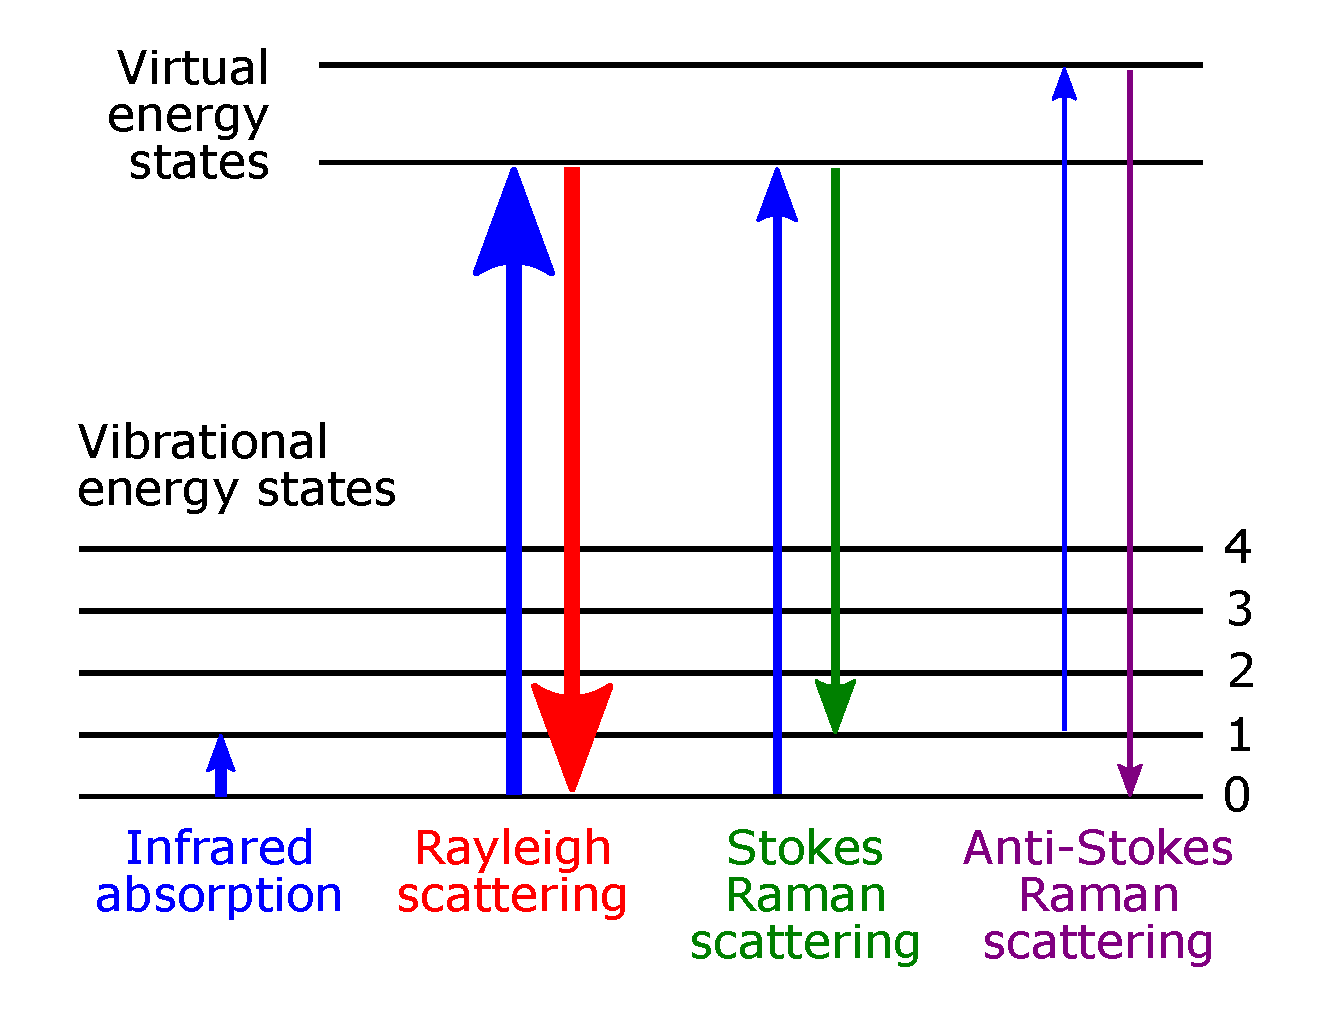
\includegraphics[width=0.7\textwidth]{energy_levels.pdf}
    \caption{Energy-level diagram showing the states involved in Raman spectra \cite{wikipedia}}
    \label{fig:energy_levels}
\end{figure}

A vibration (vibration coordinate $\rho$) is \textit{Raman active} when the polarizability $\alpha$ (or \textit{induced dipolar momentum}) of the molecule is changed (described as $\frac{\partial \alpha}{\partial \rho} \neq  \varnothing$). This illustrates that the nature of the Raman effect is physically different from the infrared. Slection rules are also different and thus lead to a different spectra \cite{Gustavo}.
\subsection{Lock-in amplifiers}
\label{sec:lock_explain}
A lock-in amplifier is a type of amplifier that extracts a signal with a known carrier wave from a noisy environment. Depending on the instrument, signals up to orders of magnitude smaller than the noise components, potentially close by in frequency, can still be reliably detected \cite{lockin}. This reliability depends on the \textit{dynamic reserve} of the instrument, which is simply a measure of how well the instrument can extract the signal when there's a much larger unwanted noise sitting on top of it. Modern instruments achieve a dynamic reserve up to \SI{120}{\decibel} \cite{lockin}.


For amplitude quantities,
\begin{equation}
	\si{\decibel} = 20 \log_{10} \left( \frac{A_{noise}}{A_{signal}}\right)
\end{equation}
So for \SI{120}{\decibel}, the above equation yields
\begin{equation}
	\SI{120}{\decibel} = 20 \log_{10} \left( \frac{A_{noise}}{A_{signal}}\right)
\end{equation}
which gives
\begin{equation}
	\frac{A_{noise}}{A_{signal}} = 10^{\frac{120}{20}} = 10^{6}
\end{equation}
So modern instruments can theoretically recover signals with an order of magnitude  $10^{-6}$ smaller than the noise.

A lock-in amplifier performs a multiplication of its input with a reference signal, also sometimes called down-mixing or heterodyne/homodyne detection, and then applies an adjustable low-pass filter to the result \cite{zurich}.This method is termed demodulation or phase-sensitive detection and isolates the signal at the frequency of interest from all other frequency components. The reference signal is either generated by the lock-in amplifier itself or provided to the lock-in amplifier and the experiment by an external source. The reference signal is usually a sine wave but could have other forms, too. Demodulation with a pure sine wave enables selective measurement at the fundamental frequency or any of its harmonics \cite{zurich}.

\begin{figure}[H]
    \centering
    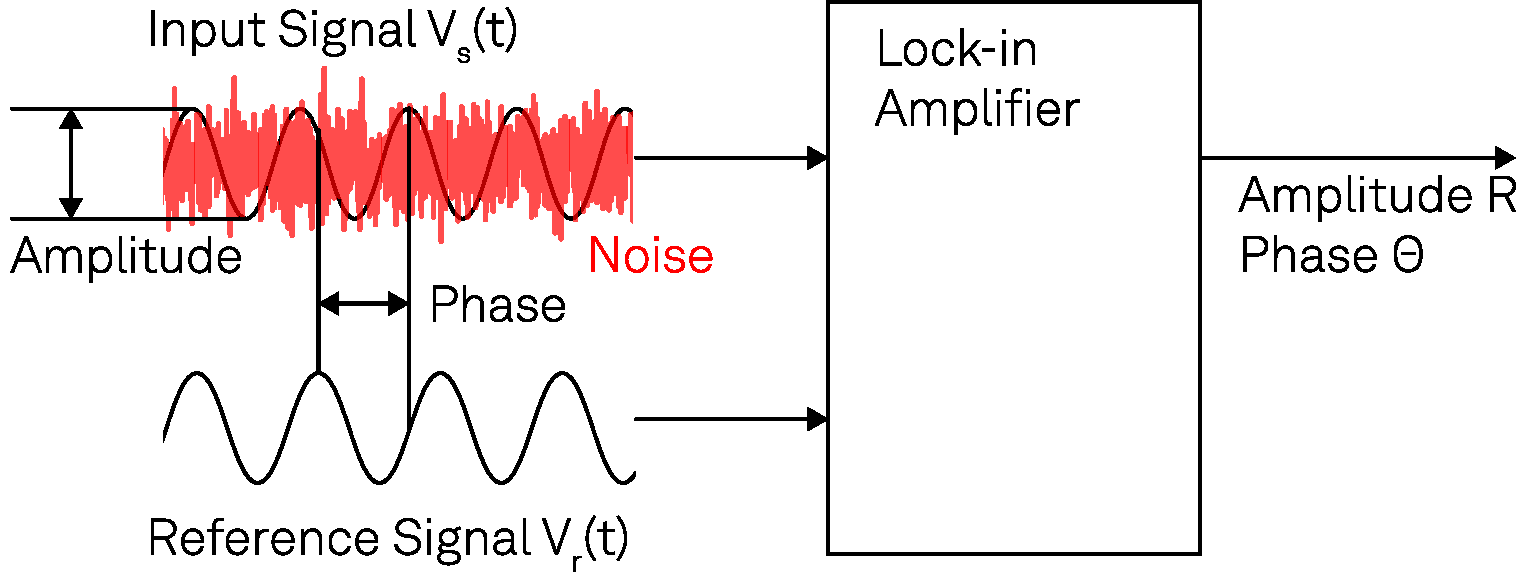
\includegraphics[width=0.7\textwidth]{lockin.pdf}
    \caption{Lock-in amplifiers are capable of measuring the amplitude and the phase of a signal relative to a defined reference signal, even if the signal is entirely buried in noise. Adapted from \cite{zurich}}
    \label{fig:lockin}
\end{figure}

\subsection{Classical and Quantum Mechanical Theory}

The classical picture of Raman scattering starts with the electric field of the incident
laser light,

\begin{equation}
    E(t) = E_0 \cos(\omega_0 t),
\end{equation}

which induces a dipole moment in the molecule,

\begin{equation}
    p(t) = \alpha E(t),
\end{equation}

where $\alpha$ is the molecular polarisability.

Since the molecule is vibrating, its polarisability can change with the normal
coordinate $Q$ of the vibration:

\begin{equation}
    \alpha(Q)
    =
    \alpha_0
    +
    \left(\frac{\partial \alpha}{\partial Q}\right)_0 Q.
\end{equation}

If the vibration has frequency $\omega_v$, the induced dipole contains
components at

\begin{equation}
    \omega_0,
    \qquad
    \omega_0-\omega_v,
    \qquad
    \omega_0+\omega_v.
\end{equation}

These correspond to:

\begin{itemize}
    \item \textbf{Rayleigh scattering:} $\omega_0$
    \item \textbf{Stokes Raman scattering:} $\omega_0-\omega_v$
    \item \textbf{anti-Stokes Raman scattering:} $\omega_0+\omega_v$
\end{itemize}

In the quantum mechanical picture, the incident photon interacts with the molecule
through a virtual state. The molecule changes its vibrational energy, and therefore
the scattered photon has a different energy:

\begin{equation}
    E_{\mathrm{out}}
    =
    E_{\mathrm{in}} \mp \hbar\omega_v.
\end{equation}

Thus, the Raman shift directly provides information about the vibrational energy
levels of the molecule.


\subsection{Polarisability}

Polarisability describes how easily the electron cloud of a molecule can be
distorted by an external electric field. The induced dipole moment is given by

\begin{equation}
    \mathbf{p}_{\mathrm{ind}}
    =
    \boldsymbol{\alpha}\mathbf{E},
\end{equation}

where $\boldsymbol{\alpha}$ is generally a tensor.

The important Raman selection rule is

\begin{equation}
    \boxed{
    \left(\frac{\partial\alpha}{\partial Q}\right)_0 \neq 0
    }
\end{equation}

A vibrational mode is therefore \textbf{Raman active if the vibration produces
a change in the molecular polarisability}.


\subsection{Degree of Depolarisation}
\label{sec:depol}
The degree of depolarisation describes how much the polarisation of the scattered
Raman light differs from that of the incident laser light. It is commonly defined as

\begin{equation}
    \rho
    =
    \frac{I_{\perp}}{I_{\parallel}},
\end{equation}

where $I_{\perp}$ is the intensity of the Raman light polarised perpendicular to
the incident polarisation and $I_{\parallel}$ is the intensity parallel to it.

For the usual treatment of Raman scattering from randomly oriented molecules,

\begin{equation}
    0 \leq \rho \leq \frac{3}{4}.
\end{equation}

A low value of $\rho$ corresponds to strongly polarised Raman scattering, whereas
a larger value indicates stronger depolarisation. The degree of depolarisation can
provide information about the symmetry of a vibrational mode.


\subsection{Scattering Cross Section}

The scattering cross section $\sigma$ describes the probability that an incident
photon will be scattered by a molecule. It can be interpreted as an effective area
that characterises the scattering probability.

Raman scattering has a very small scattering cross section compared with Rayleigh
scattering. Consequently, Raman signals are weak and require sensitive detectors
and sufficiently strong laser illumination.


\subsection{Normal Coordinates and Normal Oscillations}

A molecule can undergo many different vibrational motions. These motions can be
decomposed into independent \textbf{normal modes}.

Each normal mode has:

\begin{itemize}
    \item a characteristic pattern of atomic motion,
    \item a characteristic vibrational frequency, and
    \item a normal coordinate $Q$ describing the amplitude of the vibration.
\end{itemize}

The molecular motion can therefore be described using a set of normal coordinates,

\begin{equation}
    Q_1,Q_2,Q_3,\ldots
\end{equation}

which correspond to the different normal modes of vibration.

The dependence of the polarisability on a normal coordinate is particularly
important for Raman spectroscopy:

\begin{equation}
    \alpha(Q)
    =
    \alpha_0
    +
    \left(\frac{\partial\alpha}{\partial Q}\right)_0 Q
    + \cdots.
\end{equation}


\subsection{Induced and Permanent Dipole Moment}

A molecule may possess a \textbf{permanent dipole moment} due to an asymmetric
distribution of electric charge,

\begin{equation}
    \mathbf{p}_0 \neq 0.
\end{equation}

An external electric field can also distort the electron cloud and produce an
\textbf{induced dipole moment}:

\begin{equation}
    \mathbf{p}_{\mathrm{ind}}
    =
    \boldsymbol{\alpha}\mathbf{E}.
\end{equation}

Raman scattering originates from this induced dipole. The electric field of the
laser drives the induced dipole, which subsequently radiates the scattered light.

\subsection{Raman shift wavenumber}
\label{sec:wavenumber}
Given that energy shifts in the incident photons are not wavelenght dependent, it makes sense to express the raman spectra in a wavelenght-independent notation. Raman shift wavenumbers are the unit used to do so. The raman shift of a photon is simply
\begin{equation}
	\Delta \nu = \nu_{0} - \nu_{s}
\end{equation}
where $\nu_{0}$ is the frequency of the incident light and $\nu_{s}$ is the frecuency of the scattered light.

This way we can express raman shifts without involving laser wavelengths knowing well that raman spectra will show in the same wavenumber regarding of the laser used.
%\subsection{The Raman Effect in One Picture}

%The essential physical picture can be summarised as
%\begin{equation}
%    E(t)
%    \rightarrow
%    p(t)=\alpha(Q)E(t)
%    \rightarrow
%    \omega_0,\,
%    \omega_0-\omega_v,\,
%    \omega_0+\omega_v.
%\end{equation}

%The Raman spectrum therefore provides information about the vibrational modes of
%the molecule. In practice, the horizontal axis is usually expressed as a Raman
%shift in $\si{\per\centi\meter}$, which corresponds to the difference between the
%wavenumber of the incident laser and that of the scattered light.

%}}}
%METHODOLOGY {{{
\section{Methodology}

\subsection{Calibration of the Monochromator}

First the monochromator's transmission curves for horizontally and vertically polarized light were looked after. To do so, a Quartz Tungsten-Halogen Lamp was used. This lamp features a stable output and broadband, inchoherent illlumination in the visible and near-IR portions of the spectrum.

A polarizer was placed at the input of the monochromator as show in figure \ref{fig:polarizer}. For further analysis, it is important that both transmission curves are comparable, and hence measured with the same set parameters in the experiment (or somehow made compatible through data processing). After tweaking the parameters of the coupler and the photomultiplier high voltage supply, the following configuration was found to have enough dynamic range to record both horizontal and vertical without saturating the instrument signals:
The setup was first manipulated as to fit the output voltage obtained by horizontally polarized light best, just below the saturation point for the whole spectra. The coupler was set in $10^{-6}$, the voltage supply for the photomultiplier to $\sim\SI{300}{\V}$ and the spectra was taken from $\SI{400}{\nm}$ to $\SI{800}{\nm}$ at a speed of $\SI{5}{\nm\per\second}$.

\begin{figure}[htp]
    \centering
    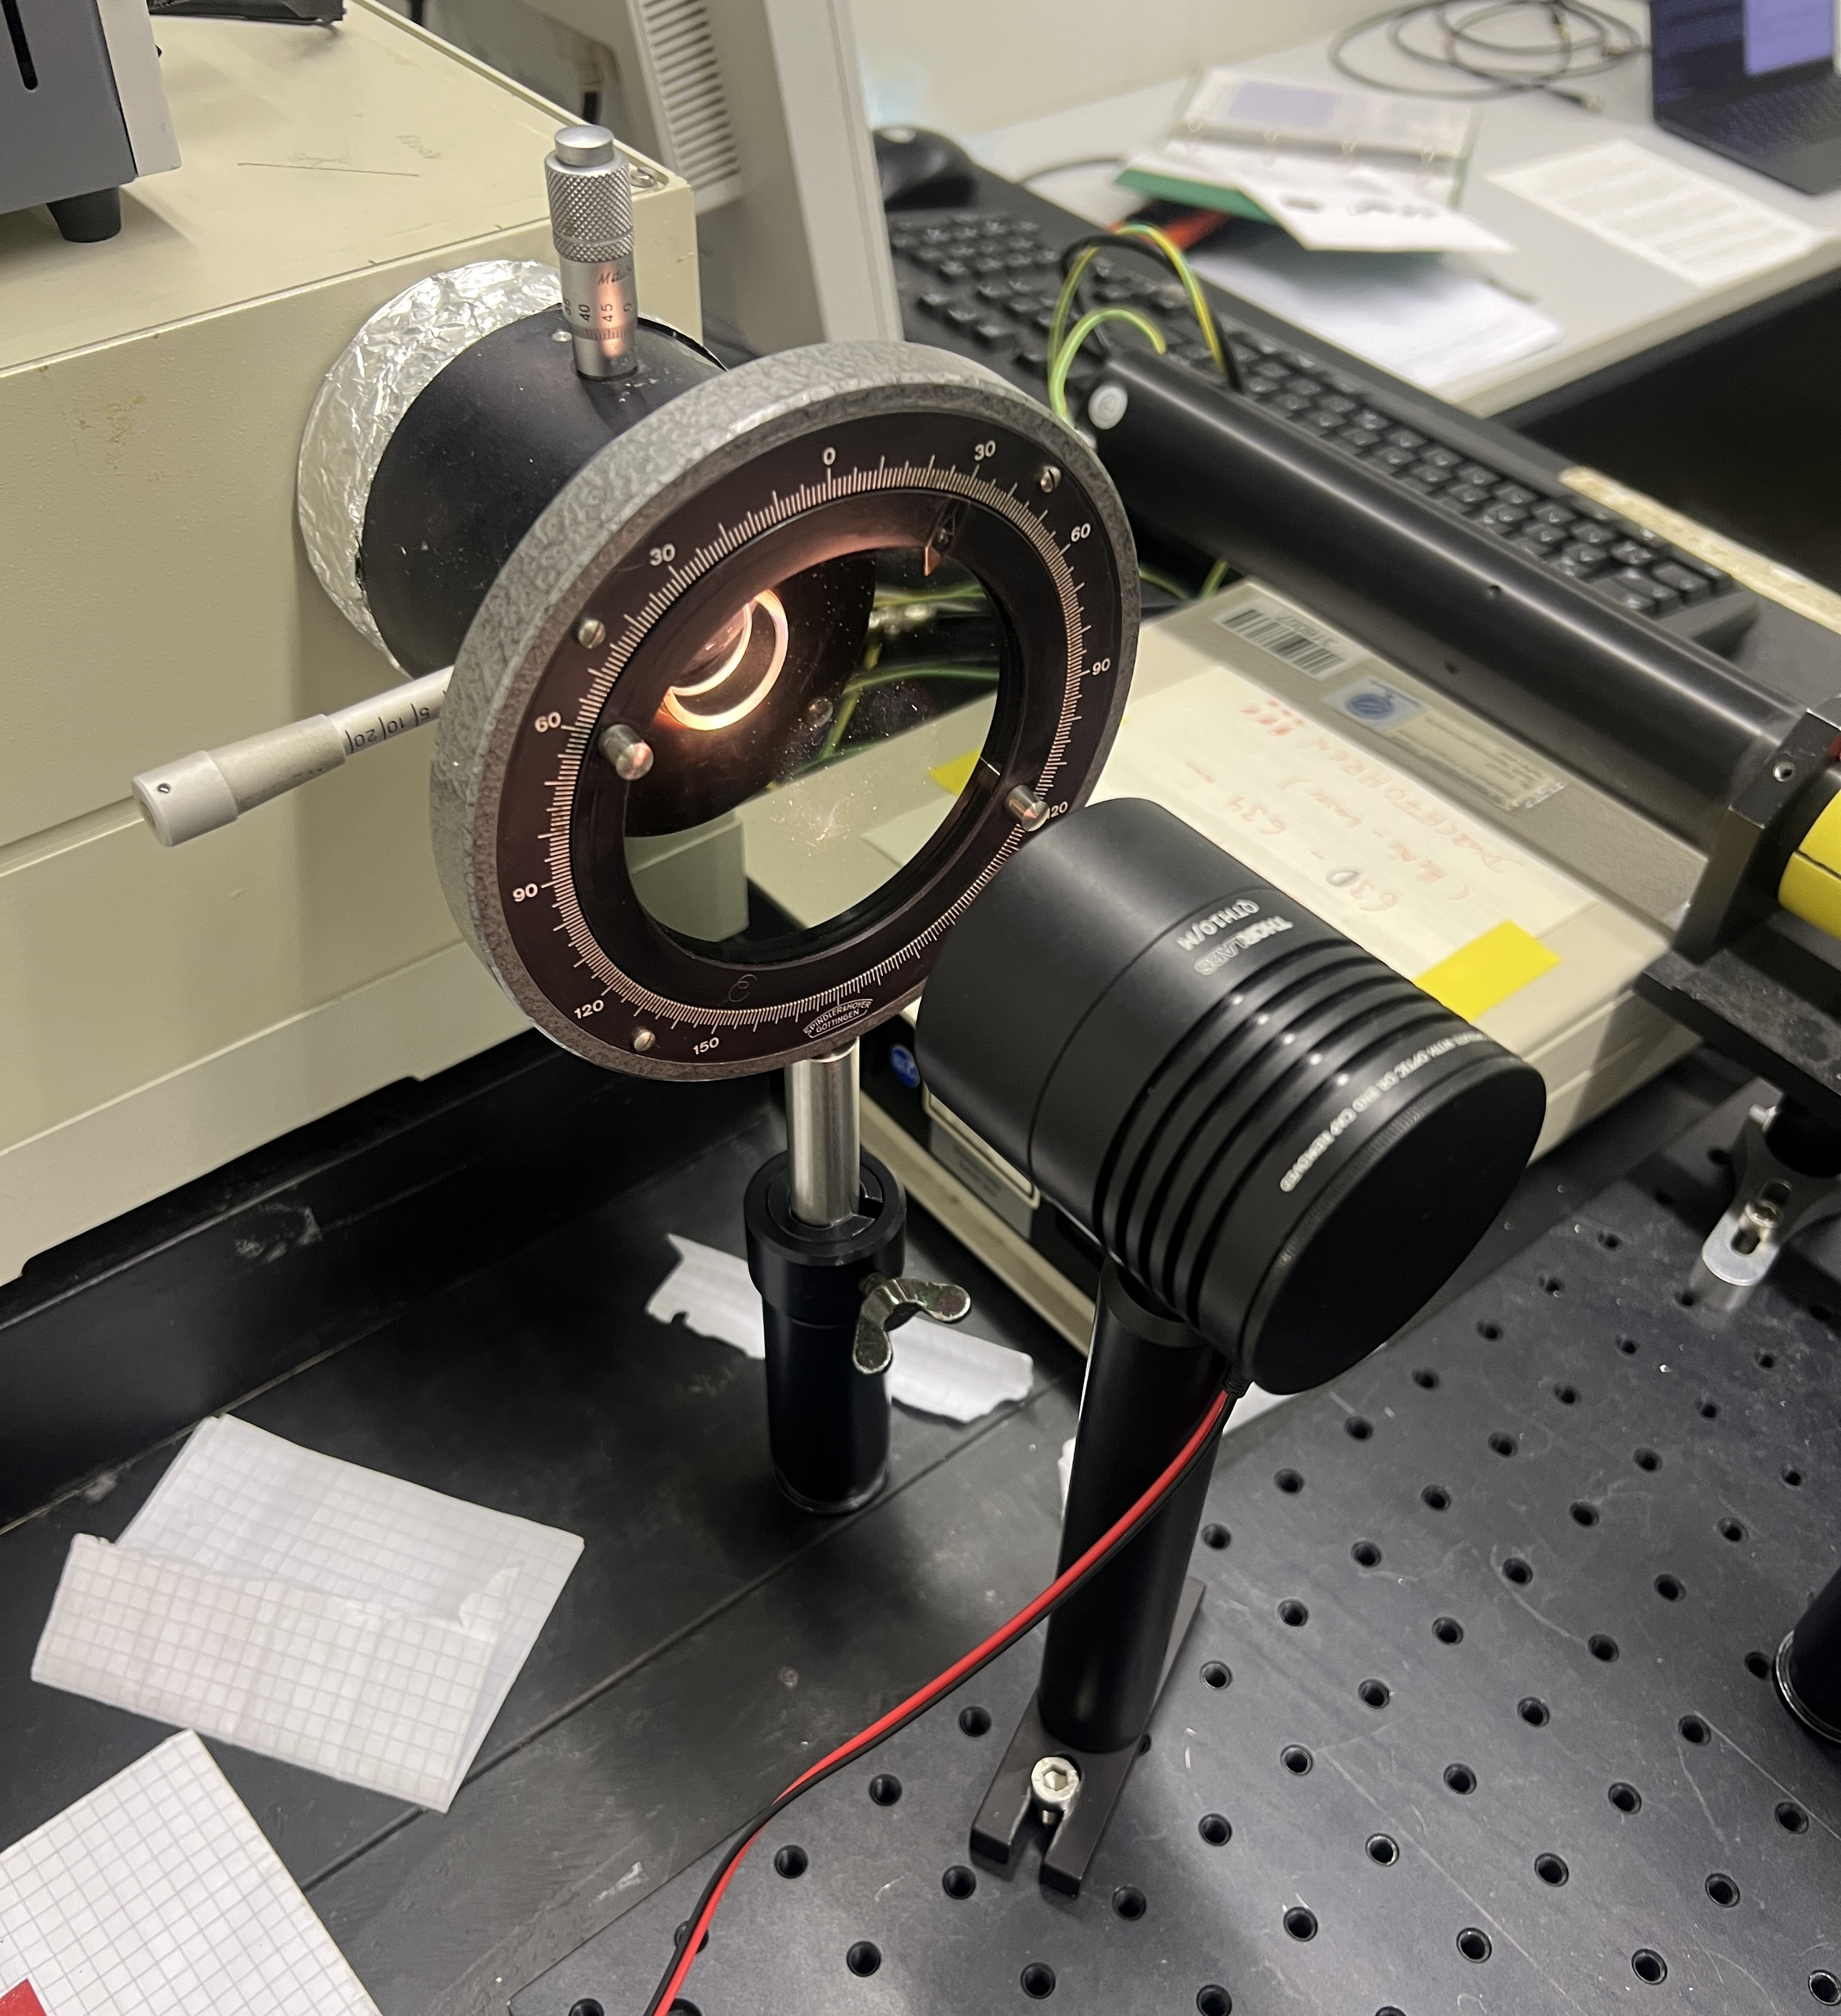
\includegraphics[width=0.5\textwidth]{polarized.jpg}
    \caption{Halogen lamp, polarizer and monochromator input}
    \label{fig:polarizer}
\end{figure}

Then, with the same set of parameters, the polarizer was vertically aligned and once again  the spectra was taken from $\SI{400}{\nm}$ to $\SI{800}{\nm}$ at the same speed.

The curve corresponding to horizontal polarization can be seen in figure \ref{fig:horizontal_raw}. The curve corresponding to vertical polarization can be seen in figure \ref{fig:vertical_raw}. Both of these figures are raw images extracted from the  TDS2001IC oscilloscope screen. 

In the experiment, the monochromator grating is adjusted by a servo motor conected to a microcontroller which was programmed to make precise adjustments to the grating. In order to know which voltage corresponds to which wavelength, the arduino's voltage output is also recorder in the oscilloscope to match the data. 
\begin{figure}[H]
    \centering
    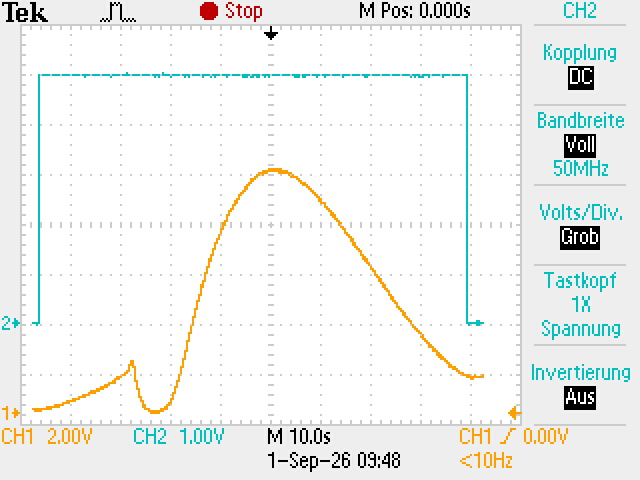
\includegraphics[width=0.7\textwidth]{horizontal_raw.jpg}
    \caption{Voltage curve of the photomultiplier for horizontally polarized light (orange) and servo voltage (blue).}
    \label{fig:horizontal_raw}
\end{figure}
\begin{figure}[H]
    \centering
    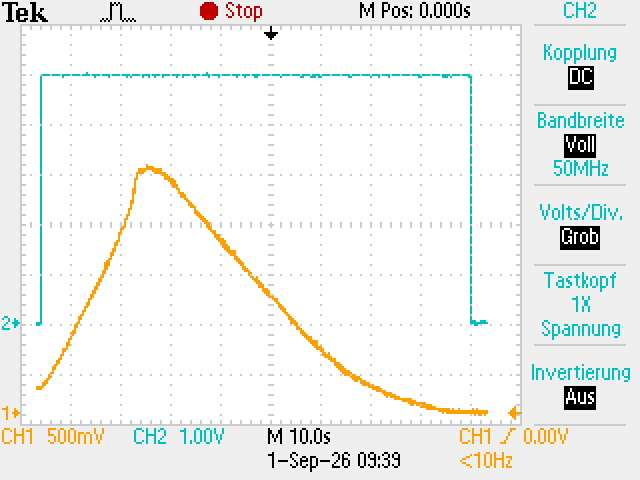
\includegraphics[width=0.7\textwidth]{vertical_raw.jpg}
    \caption{Voltage curve of the photomultiplier for vertically polarized light (orange) and servo voltage (blue).}
    \label{fig:vertical_raw}
\end{figure}

The data shown in both figures \ref{fig:horizontal_raw} and \ref{fig:vertical_raw} will be useful to apply instrument response correction (correct the actual raman spectra taking into account the wavelength-dependent intensity of the photocromator).


The Halogen lamp was removed from the array, and the two lenses that form the telescope were placed so that the laser light goes in as focused as possible in the monochromator.
The ethanol + salt sample was inserter in the chamber. This sample has a very strong rayleigh reflection, and is thus the ideal sample to align the experiment. The monochromator was swept in between 622 and 642 nm. The Voltage curve can be seen in figure \ref{fig:base}. Note that the lock-in mechanism and the chopper are not active yet.

\begin{figure}[H]
    \centering
    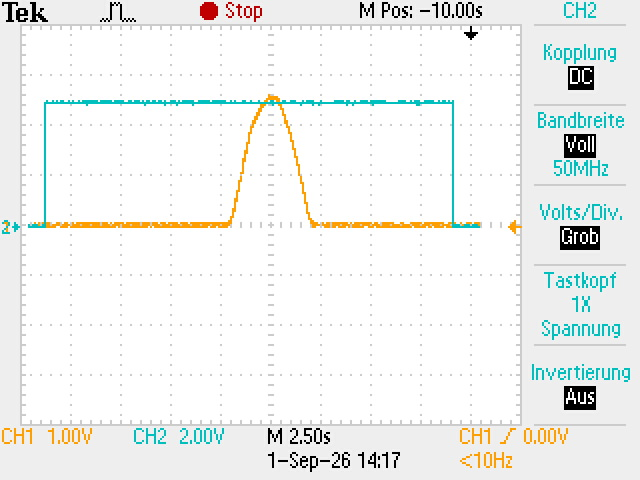
\includegraphics[width=0.7\textwidth]{base.jpg}
    \caption{Voltage curve of the \SI{633}{\nano\meter} laser (ethanol +salt cuvette)}
    \label{fig:base}
\end{figure}

Figure \ref{fig:base} shows that our laser indeed has a gaussian profile with a peak pressumably at \SI{633}{\nano\meter}.




\subsubsection{instrument response correction}
\label{sec:correction}
Figures \ref{fig:horizontal_raw} and \ref{fig:vertical_raw} prove that the monochromator has a wavelength-dependent response $R(\lambda)$, thus we can say that approximately
\begin{equation}
	I_{measured}(\lambda) = I_{true}(\lambda)R(\lambda)
\end{equation}

So to correct the measured spectrum we divide by the response of the monochromator.


\subsection{Experiment Setup}

Having the monochromator response, the rest of the setup can be properly introduced in the experiment. A laser of wavelength of \SI{633}{\nano\meter} goes through a mechanical chopper whose frecuency can be adjusted by a control box. The laser then goes through a cage system containing a sample, it is then reflected onto the telescope system. Finally the laser goes inside the photochromator. the photomultiplier then outputs a signal for data analysis.
 In between the sample and the monochromator, a polarizer is introduced to analize the change in light polarization after the sample. The laser polarization can also be adjusted by rotating the laser tube.

 A diagram of the experiment can be seen in \ref{fig:setup}.

\begin{figure}[H]
    \centering
    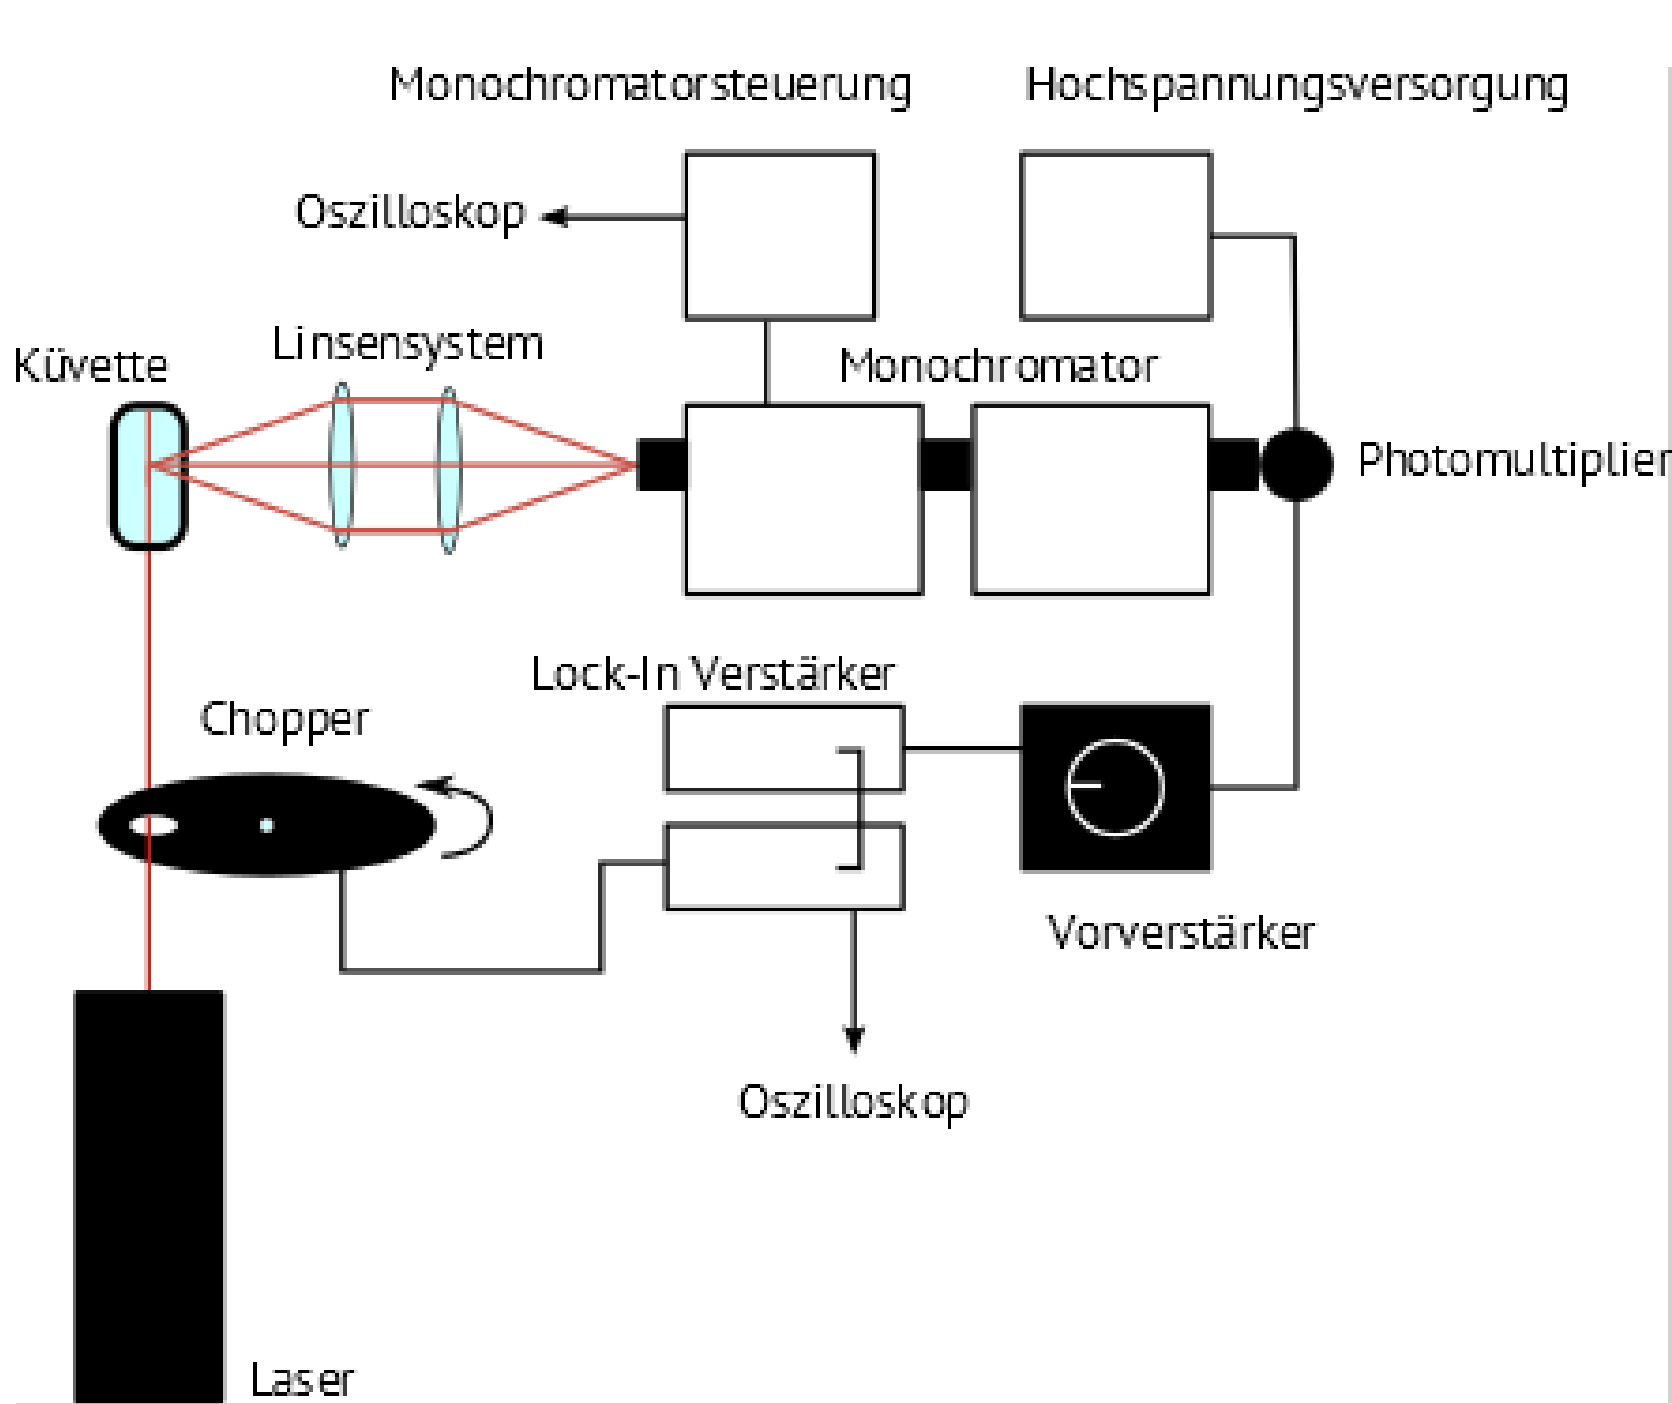
\includegraphics[width=0.7\textwidth]{setup.png}
    \caption{Setup of the experiment. Taken from \cite{manual}}
    \label{fig:setup}
\end{figure}


After the monochromator, the signal processing electronics take place. Given that the photomultiplier signal is very small, immediately after a preamp is connected to strengthen the signal. Said signal is then fed to a phase sensitive Detector. This detector has as reference the phase-shifted signal of the chopper. A picture of this part of the array is seen in figure \ref{fig:filters}. These electronics and configuration is explained in detail in section \ref{sec:configuration_locking}

\begin{figure}[H]
    \centering
    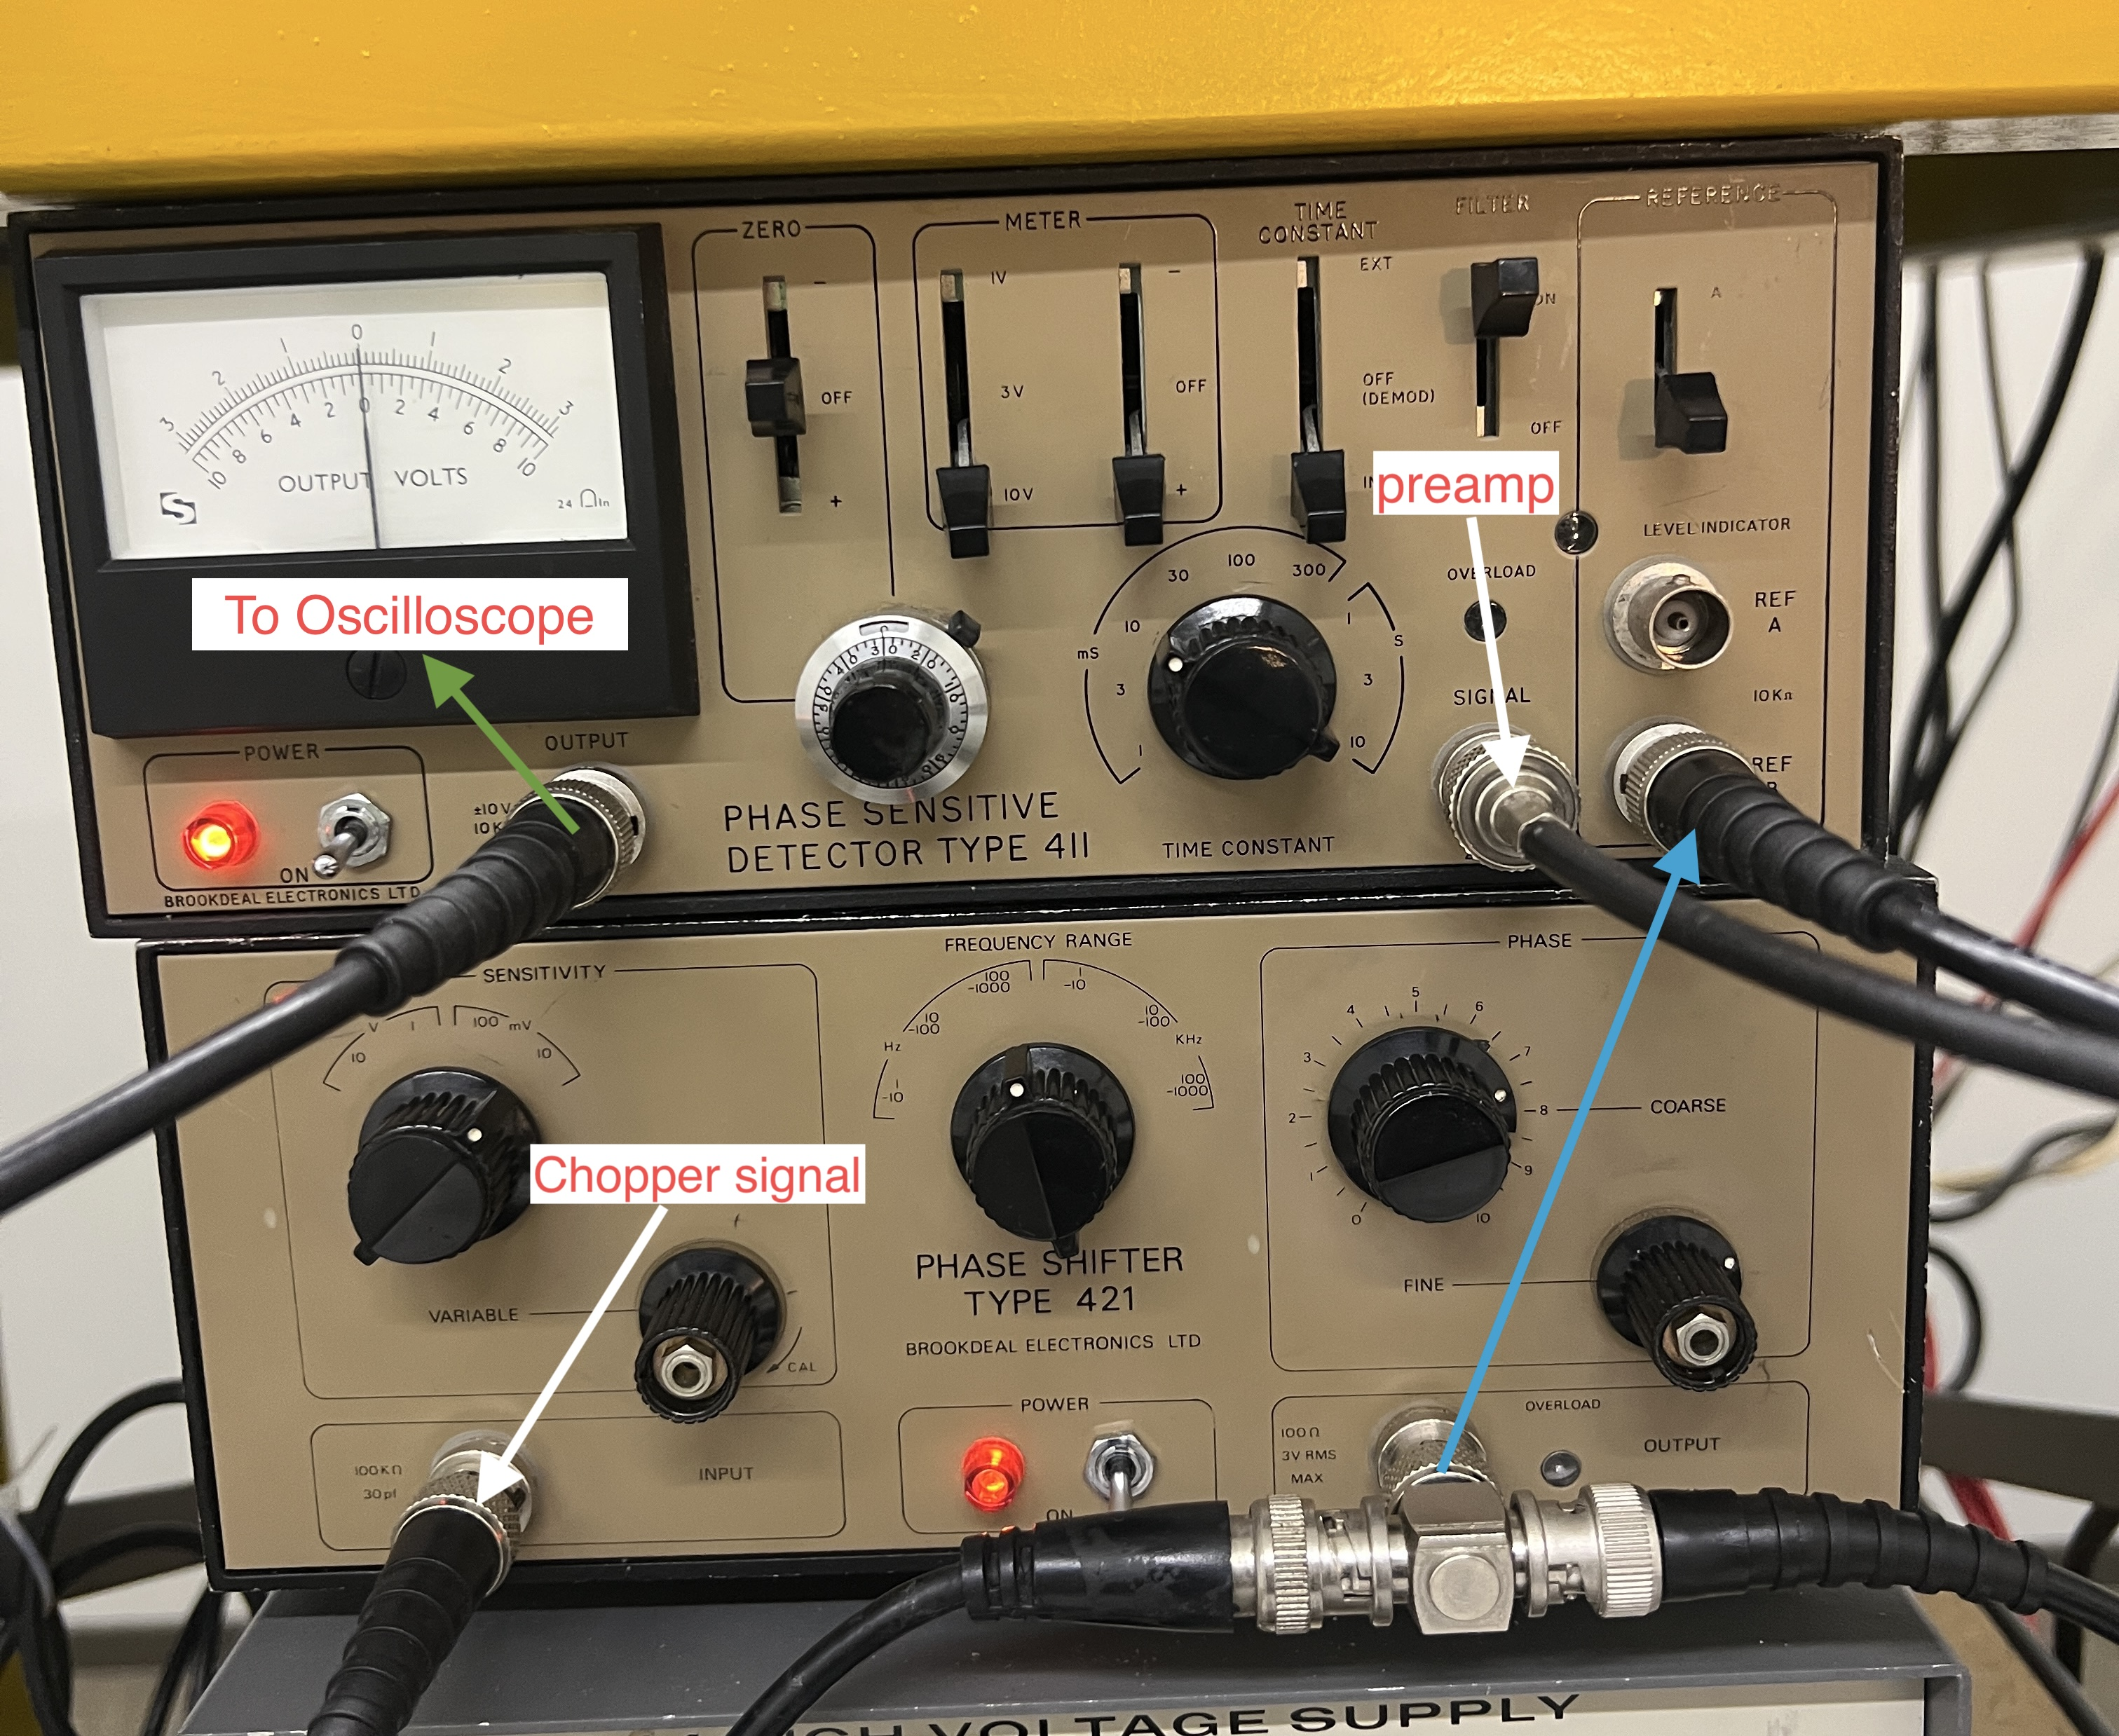
\includegraphics[width=0.7\textwidth]{filters.jpg}
    \caption{Lock-In amplifier inputs and outputs (knobs are not in final position)}
    \label{fig:filters}
\end{figure}


\subsection{Lock-In Amplifier}
It will be seen in the following sections of this protocol that raman peaks are of very low intensity and can be hard to discern in a regular spectrum; this is because raman scattering is considerably weaker than rayleigh scattering. Often they can be burried in noise and the rayleigh peaks can also bury them if they're overlapping.

To overcome this challenge, we need a way to remove unwanted noise from the spectra. This is where the Lock-In amplifier comes in handy as explained in section \ref{sec:lock_explain}
\subsubsection{Lock-in amplifier configuration}
\label{sec:configuration_locking}
The optical chopper was set to an arbitrary frecuency (around \SI{130}{\Hz}). The chopper driver generates an AC output that was forwared to our Phase shifter. The output of the phase shifter is then taken as a reference signal in the phase sensitive detector (PSD). Furthermore, the chopper frecuency can be calculated with the AC output signal. The output of the current amplifier (whose input is the photomultiplier) is then taken as the input signal on the PSD. Refer to figure\ref{fig:filters} for a visual image of the connections.


The fine-tuning of the lock-in mechanism took place. Given that the chopper has a frencuency of around \SI{130}{\Hz}, the phase shifter fricuency has to be set accordingly to the range $100 - 1000 \si{Hz}$. Then the phase shift is adjusted either to match closely either $0^{\circ}$ or $180^{\circ}$. This is because the photodiode signal at the chopping frequency has the form
\begin{equation}
	S(t) = A \cos(\omega t + \phi)
\end{equation}
while the reference from the chopper is
\begin{equation}
	R(t) = \cos(\omega t + \theta)
\end{equation}

At the PSD, both signals are multiplied and low-pass filtered, giving an expression ressembling
\begin{equation}
	V(t) = \frac{A}{2}\cos(\phi - \theta)
\end{equation}
It is evident that the resulting signal has an absolute maxima when the above condition is met. In practice, this is done by hooking the photodiode and the phase-shifted chopper signal in the two channels of the oscilloscope and adjusting the time scale to distinguish the square oscillating signal as seen in figure \ref{fig:locking}

\begin{figure}[H]
    \centering
    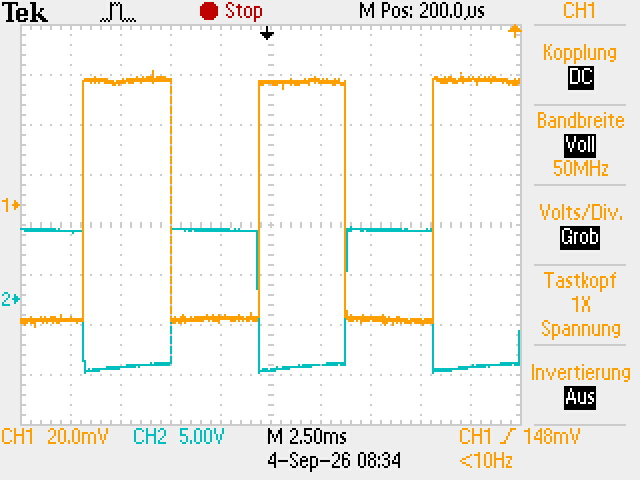
\includegraphics[width=0.7\textwidth]{lockin.jpg}
    \caption{Phase shifted chopper (blue) and photodiode (yellow) on the oscilloscope. They fulfill the locked condition }
    \label{fig:locking}
\end{figure}

The time constant $\alpha$ of the PSD was introduced after that. The time constant is the low pass constant which determines how quickly the PSD output is allowed to respond to changes by controlling the bandwidth of its low pass filter.

Simply put, if $\alpha$ is small, the output responds quickly, but more noise gets through. Viceversa, if $\alpha$ is big, output changes slowly, but more noise is rejected.

% }}}
% Results {{{1
\section{Results}
% Calibration {{{2
After processing the data by taking into account the servo response, both of the curves seen in  figures \ref{fig:horizontal_raw} and \ref{fig:vertical_raw} are now shown with the wavelength (\si{\nano\meter}) in figures \ref{fig:horizontal_processed} and \ref{fig:vertical_processed}

\begin{figure}[H]
    \centering
    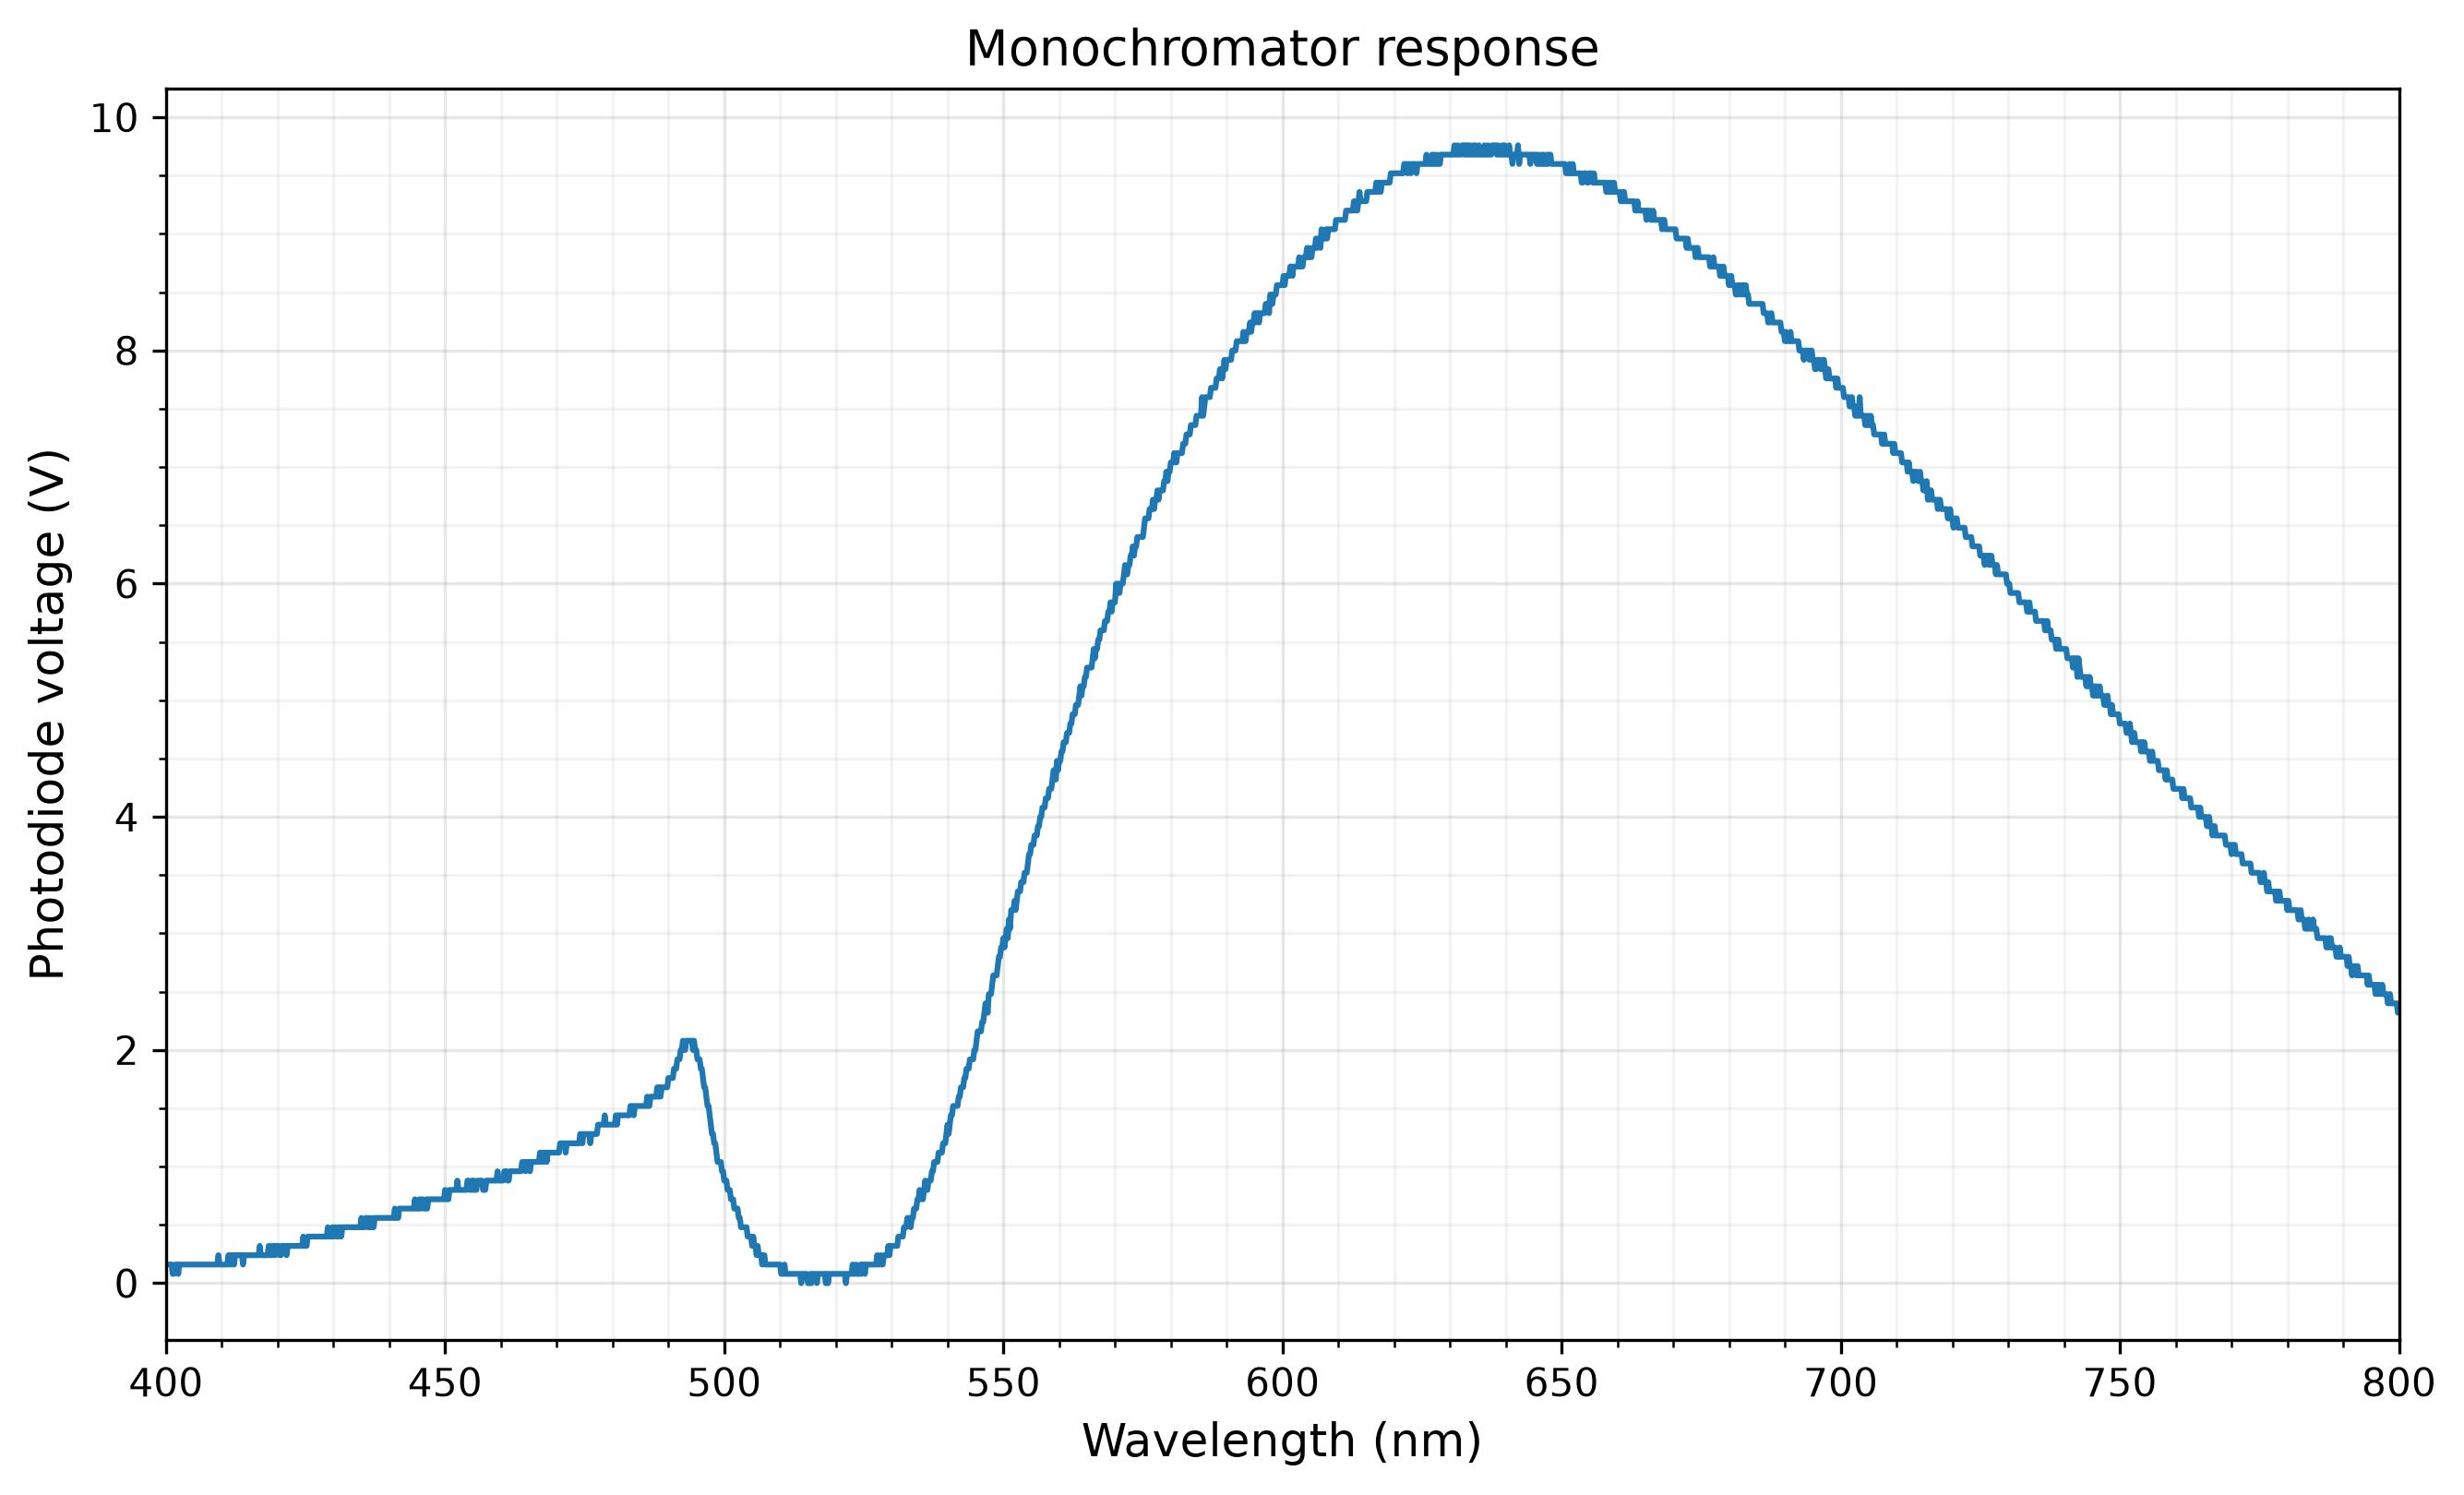
\includegraphics[width=0.7\textwidth]{horizontal_processed.jpg}
    \caption{Monochromator response (horizontally polarized light).}
    \label{fig:horizontal_processed}
\end{figure}
\begin{figure}[H]
    \centering
    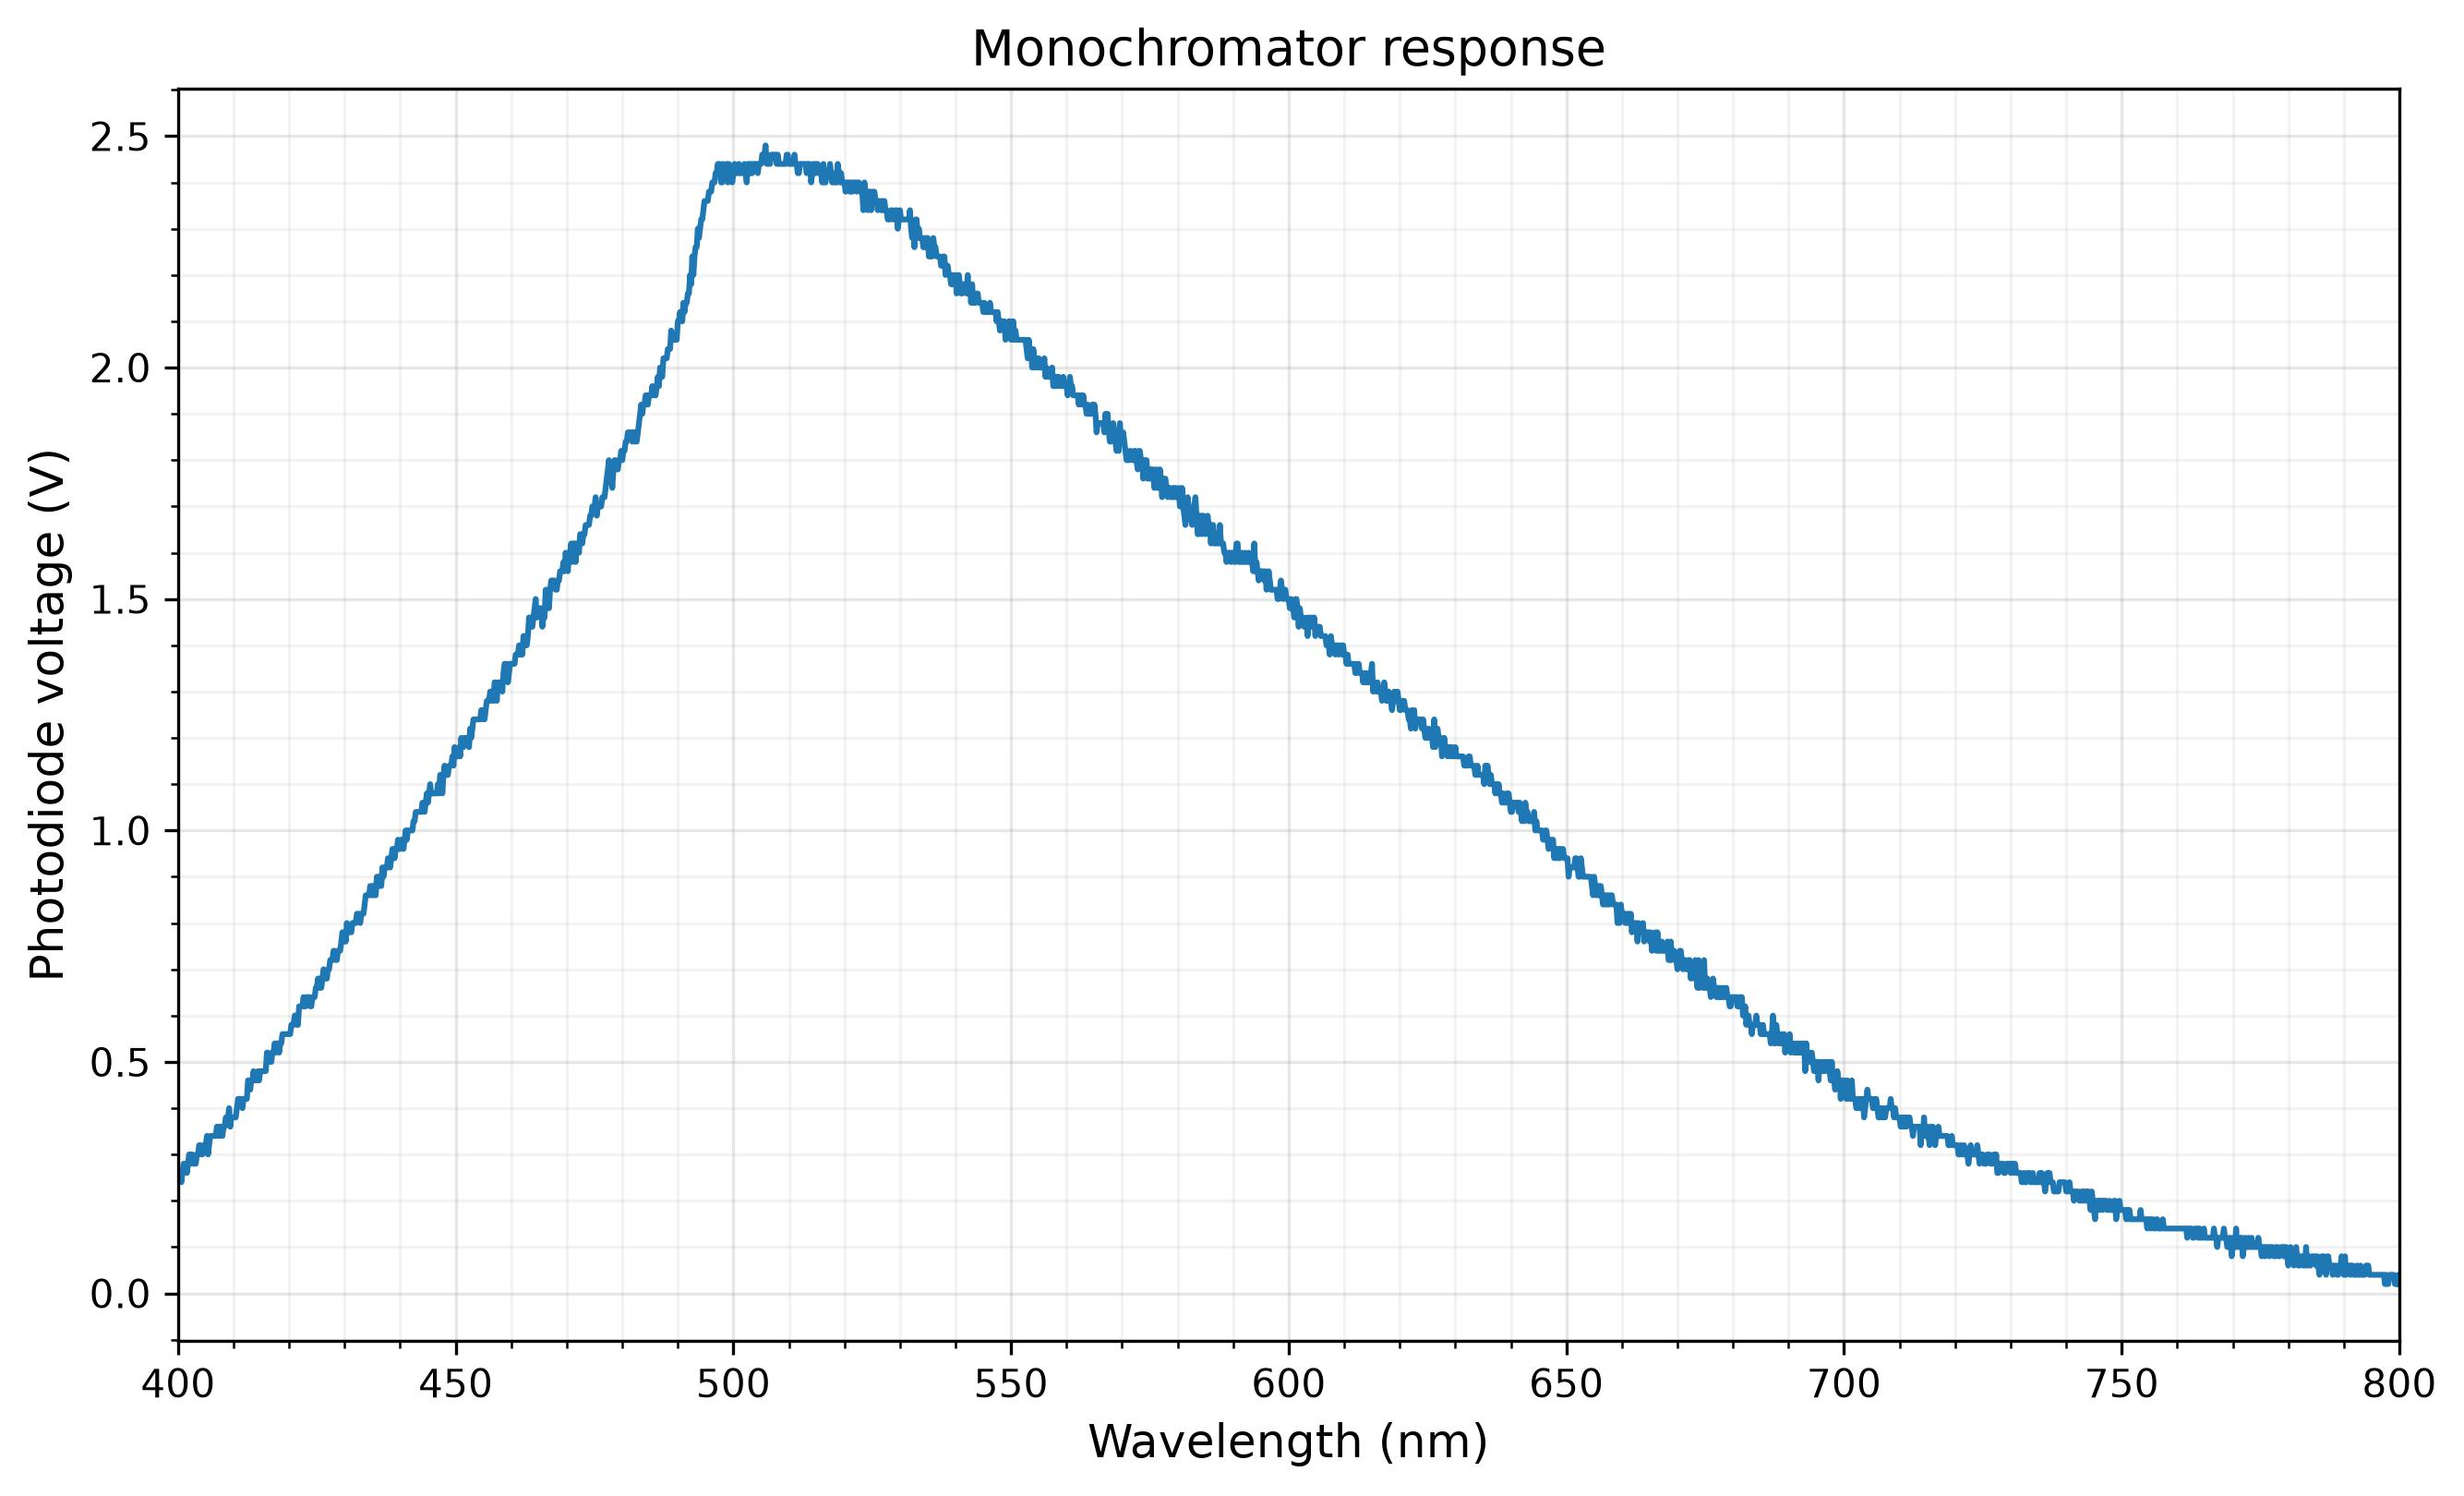
\includegraphics[width=0.7\textwidth]{vertical_processed.jpg}
    \caption{Monochromator response (vertically polarized light).}
    \label{fig:vertical_processed}
\end{figure}

\begin{figure}[H]
    \centering
    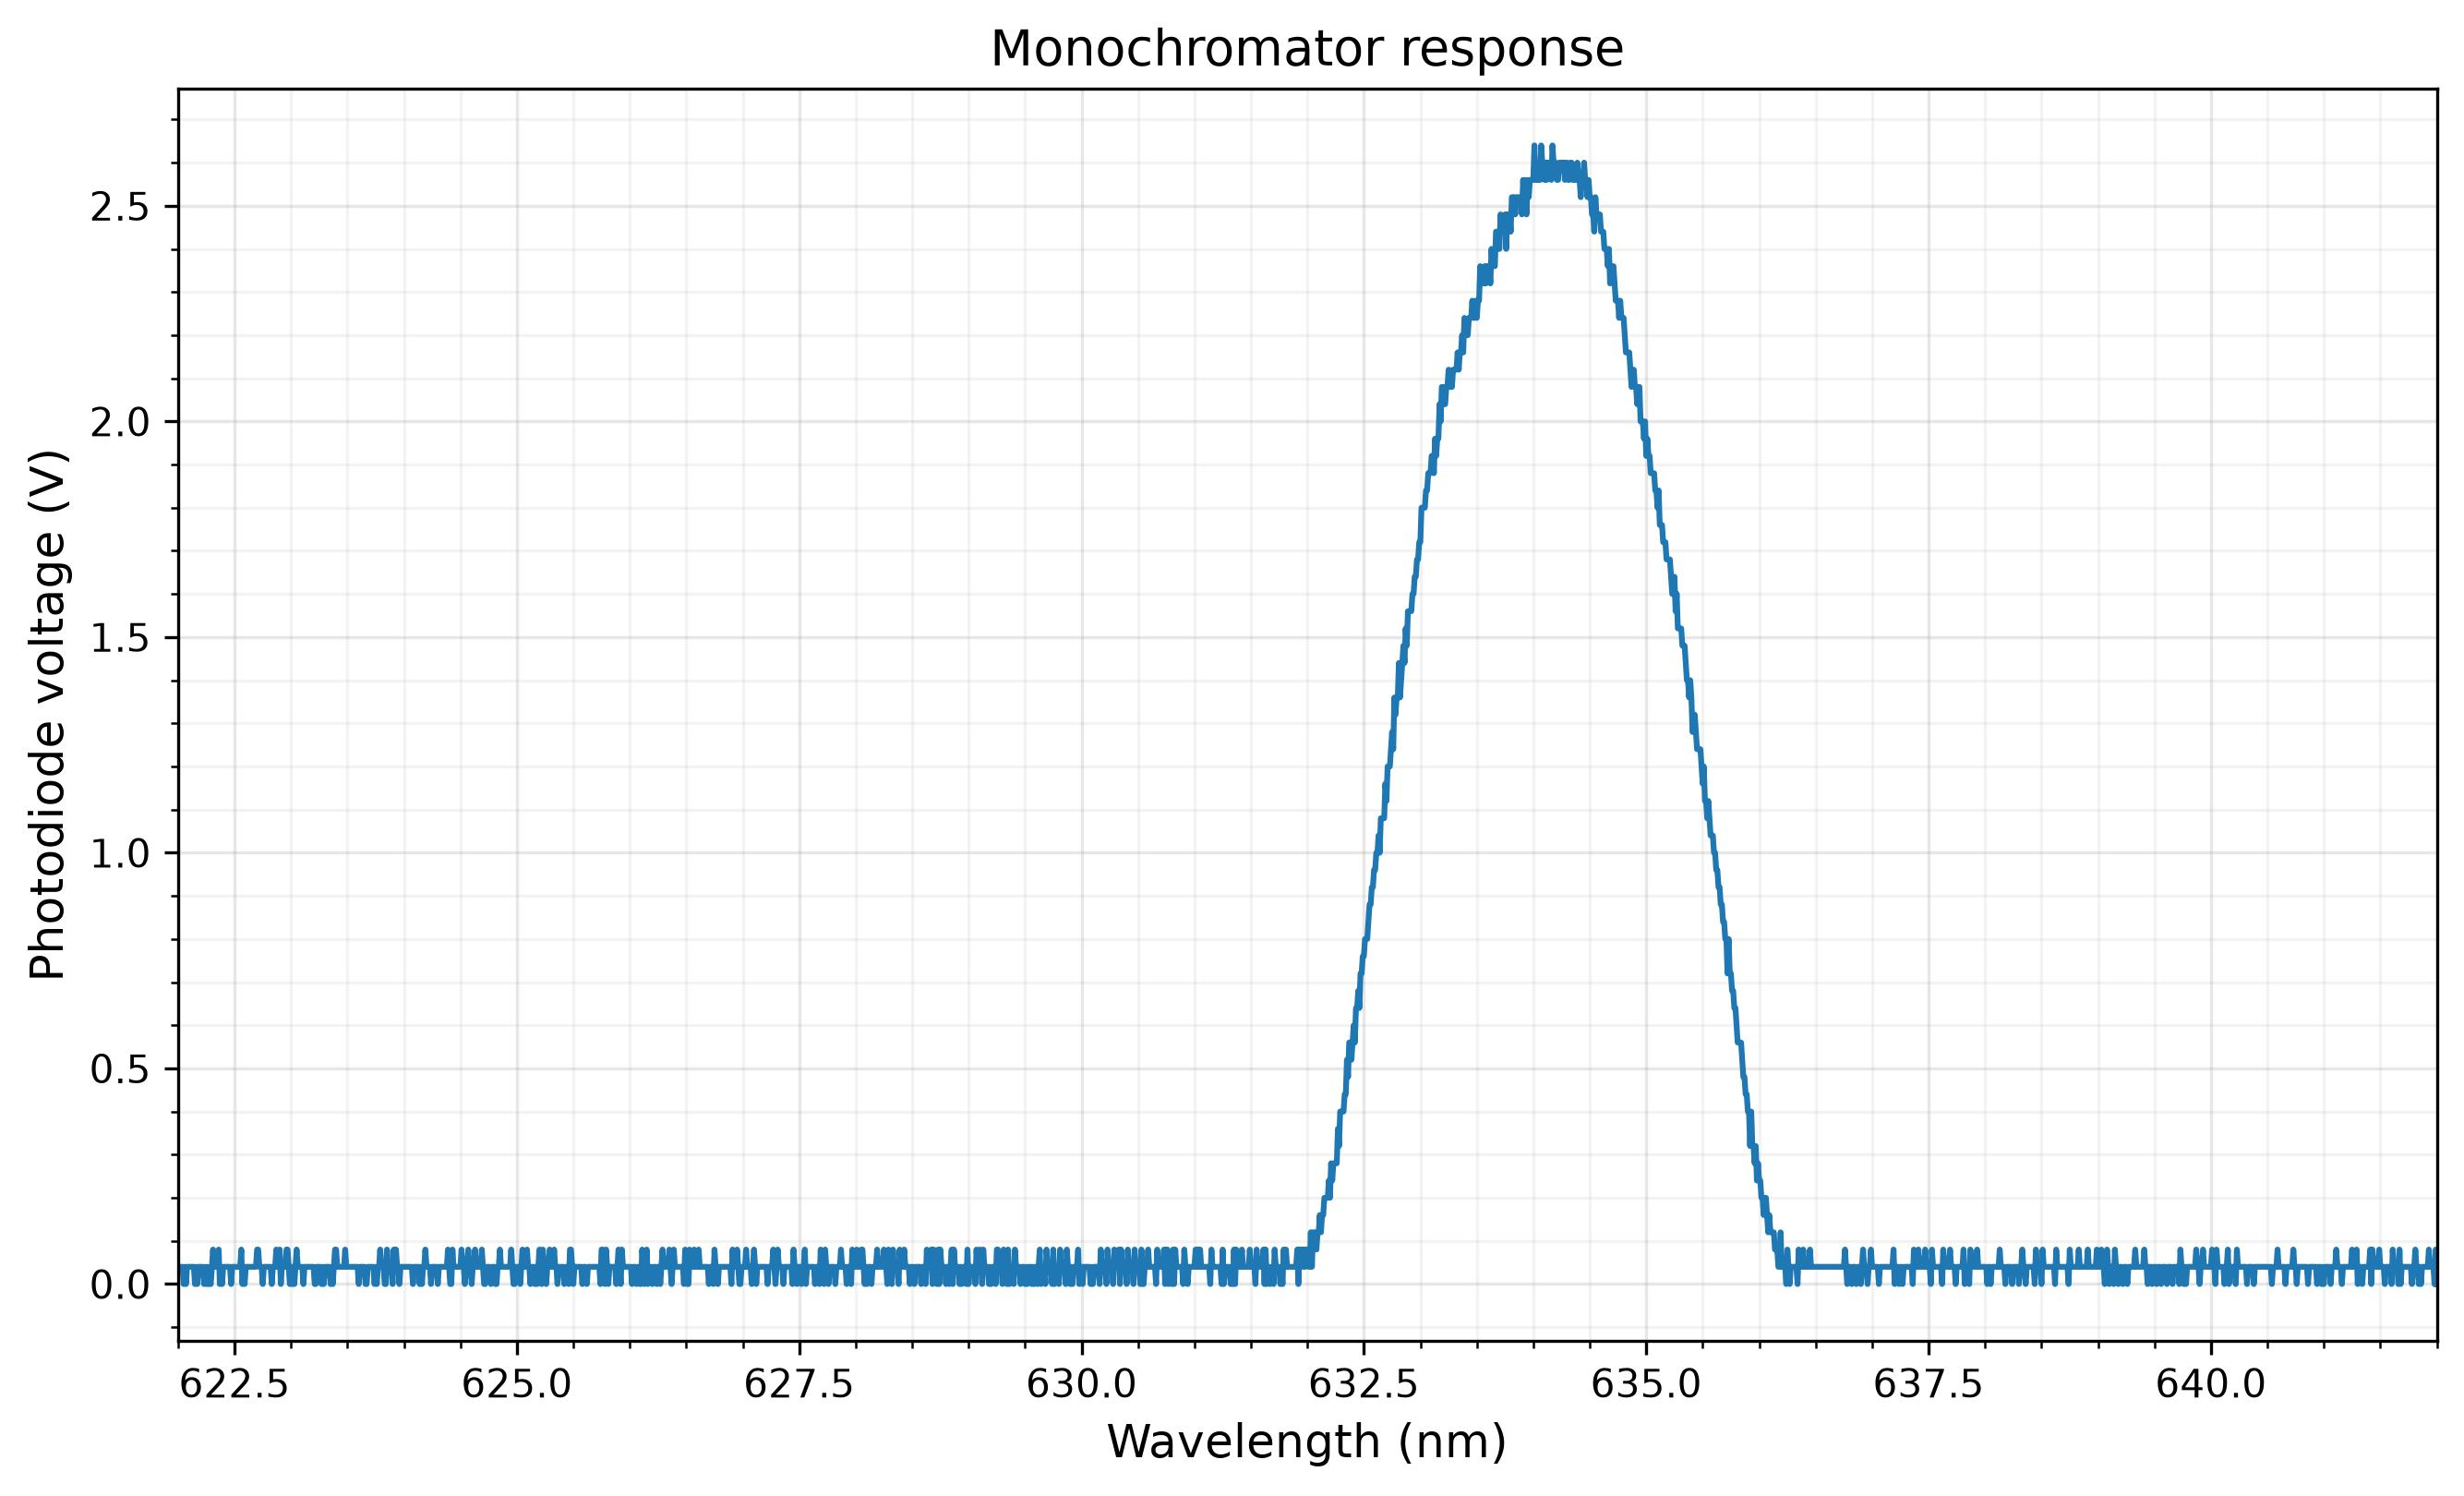
\includegraphics[width=0.7\textwidth]{base_processed.jpg}
    \caption{Laser spectra (ethanol + salt)}
    \label{fig:base_processsed}
\end{figure}

Take note that all of the next results are corrected to consider the monochromator polarizability/wavelength response as explained in section \ref{sec:correction}.
% }}}2
% Spectra of CCL4 and Benzene {{{2
\subsection{Raman spectra of CCL4 and Benzene}
As suggested in  section \ref{sec:wavenumber}, all of the results are presented in the appropiate raman shift wavenumber.

%----------------CCL4-----------------------%
\begin{figure}[H]
    \centering
    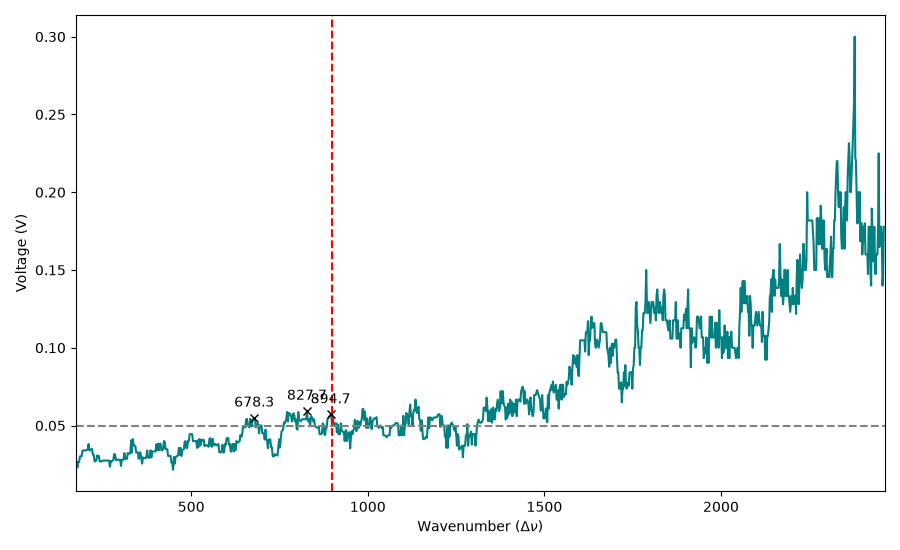
\includegraphics[width=0.7\textwidth]{plots/CCL4_0_0.png}
    \caption{CCL4 spectra with laser at $0^{\circ}$ and polarizer at $0^{\circ}$}
    \label{fig:CCL4_0_0}
\end{figure}

\begin{figure}[H]
    \centering
    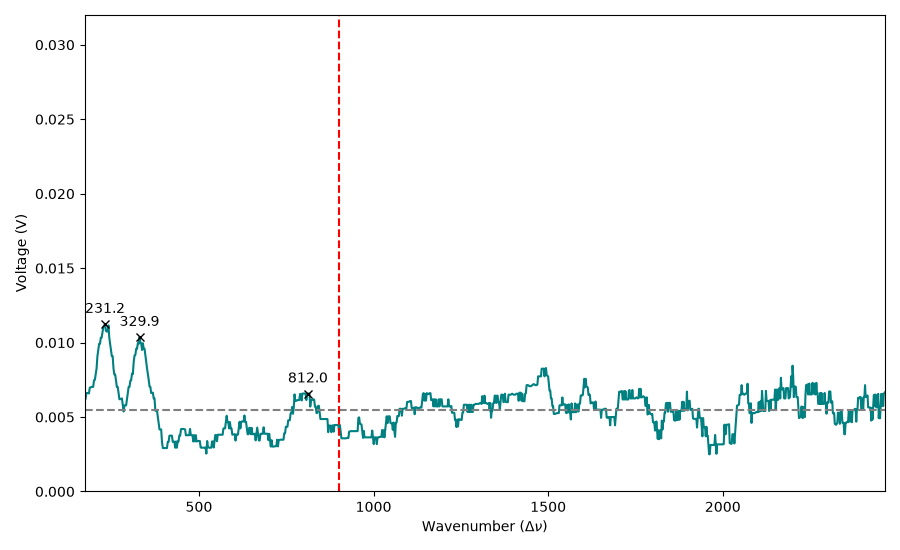
\includegraphics[width=0.7\textwidth]{plots/CCL4_0_90.png}
    \caption{CCL4 spectra with laser at $0^{\circ}$ and polarizer at $90^{\circ}$}
    \label{fig:CCL4_0_90}
\end{figure}

\begin{figure}[H]
    \centering
    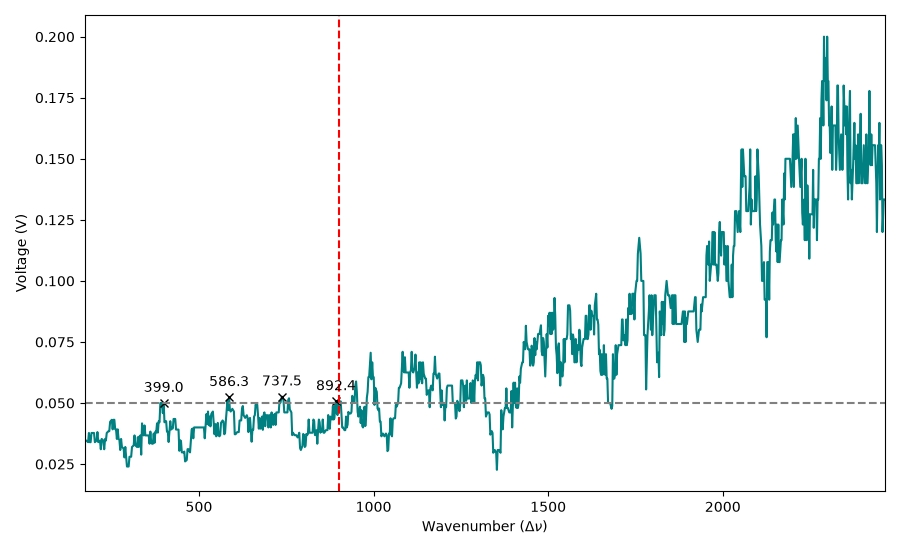
\includegraphics[width=0.7\textwidth]{plots/CCL4_90_0.png}
    \caption{CCL4 spectra with laser at $90^{\circ}$ and polarizer at $0^{\circ}$}
    \label{fig:CCL4_90_0}
\end{figure}

\begin{figure}[H]
    \centering
    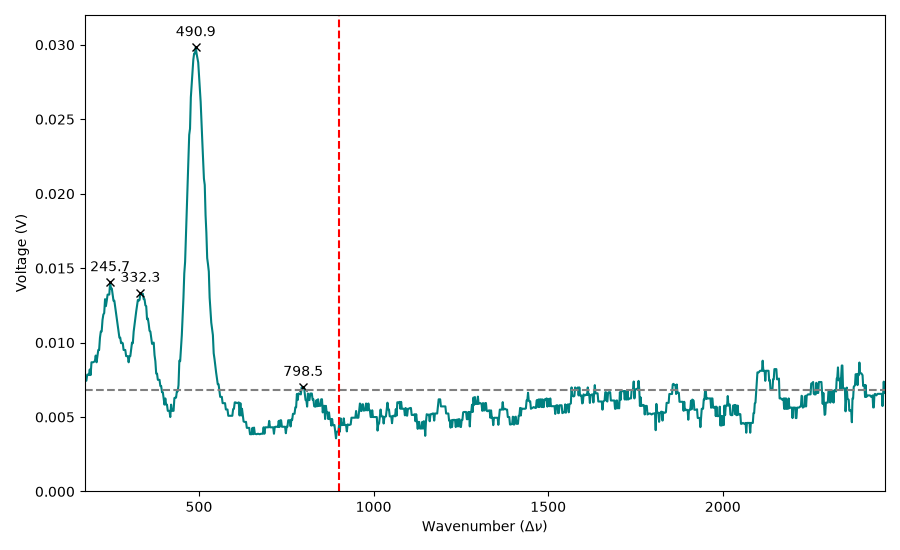
\includegraphics[width=0.7\textwidth]{plots/CCL4_90_90.png}
    \caption{CCL4 spectra with laser at $90^{\circ}$ and polarizer at $90^{\circ}$}
    \label{fig:CCL4_90_90}
\end{figure}

%----------------Benzene-----------------------%
\begin{figure}[H]
    \centering
    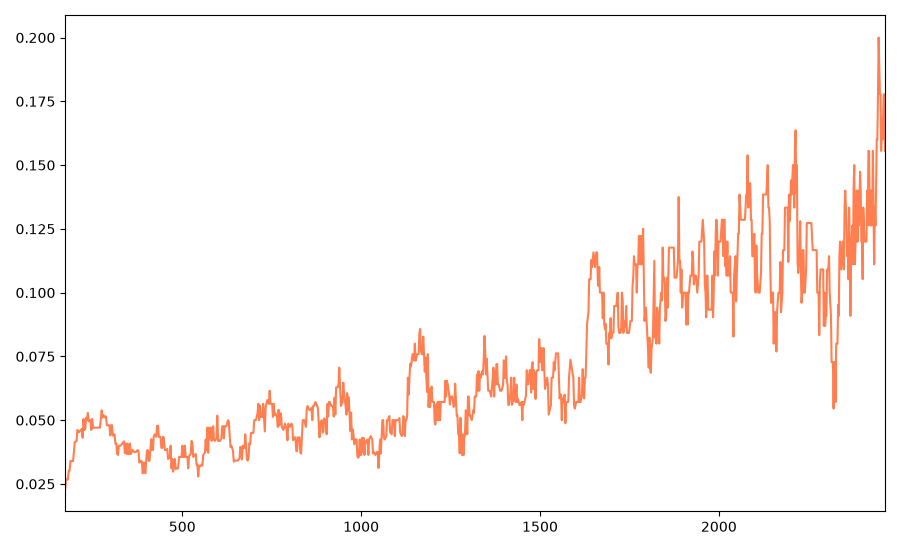
\includegraphics[width=0.7\textwidth]{plots/benzene_0_0.png}
    \caption{Benzene spectra with laser at $0^{\circ}$ and polarizer at $0^{\circ}$}
    \label{fig:benzene_0_0}
\end{figure}

\begin{figure}[H]
    \centering
    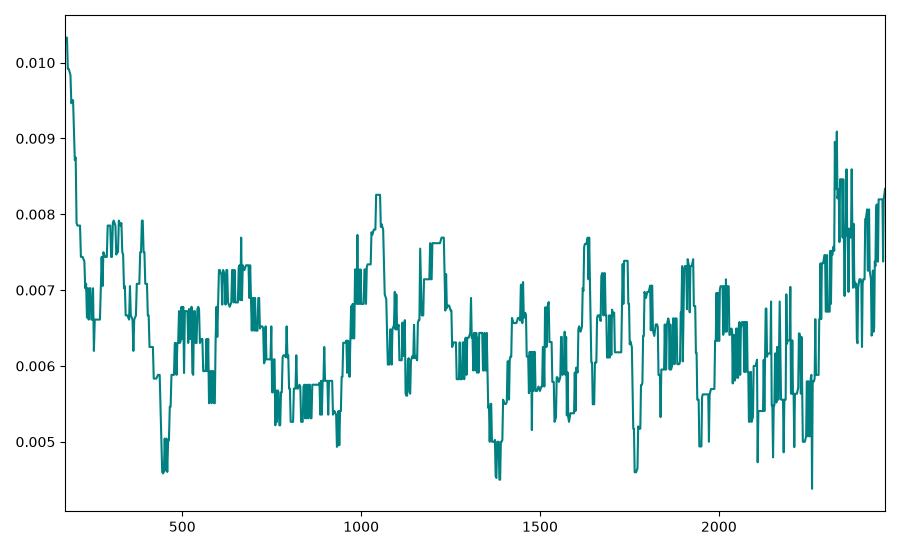
\includegraphics[width=0.7\textwidth]{plots/benzene_0_90.png}
    \caption{Benzene spectra with laser at $0^{\circ}$ and polarizer at $90^{\circ}$}
    \label{fig:benzene_0_90}
\end{figure}

\begin{figure}[H]
    \centering
    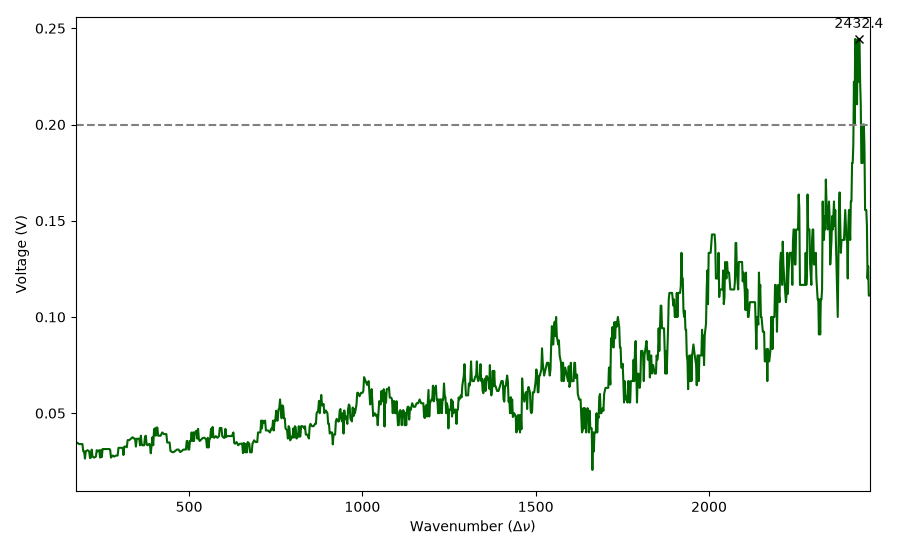
\includegraphics[width=0.7\textwidth]{plots/benzene_90_0.png}
    \caption{Benzene spectra with laser at $90^{\circ}$ and polarizer at $0^{\circ}$}
    \label{fig:benzene_90_0}
\end{figure}

\begin{figure}[H]
    \centering
    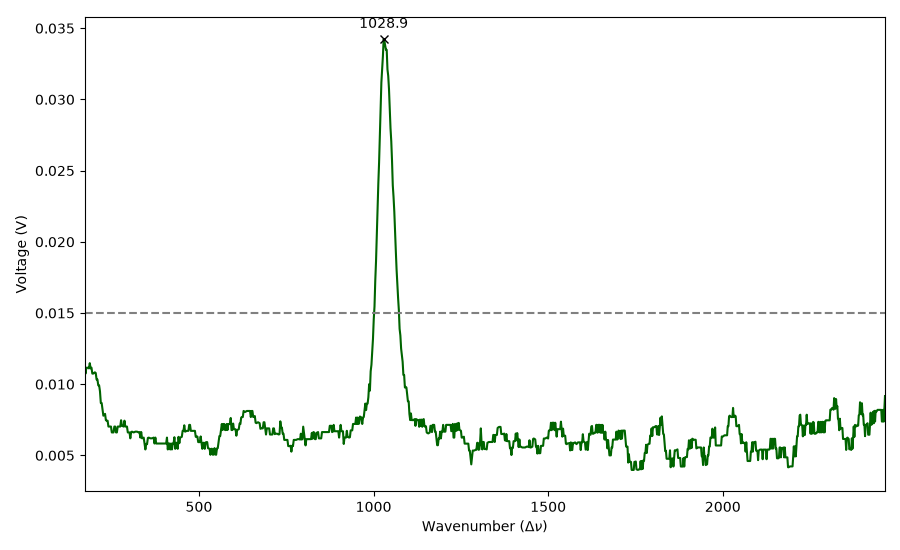
\includegraphics[width=0.7\textwidth]{plots/benzene_90_90.png}
    \caption{Benzene spectra with laser at $90^{\circ}$ and polarizer at $90^{\circ}$}
    \label{fig:benzene_90_90}
\end{figure}
% }}}2
% unknown spectra {{{2
\subsection{Unknown sample Spectra}
Figures \ref{fig:unknown_1} and \ref{fig:unknown_2} show the spectra recorded for two samples whose content was not known in advance.

\begin{figure}[H]
    \centering
    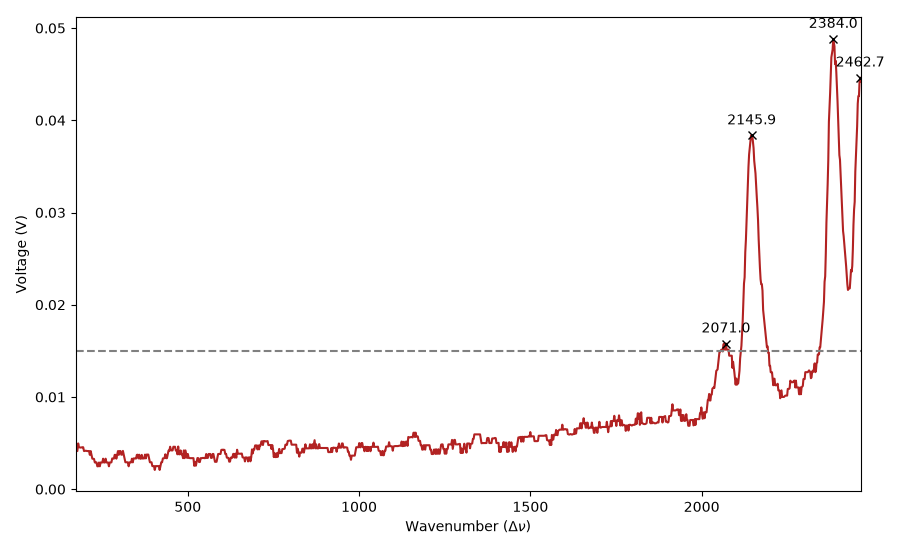
\includegraphics[width=0.7\textwidth]{plots/unknown_1.png}
    \caption{Spectra of \textit{unknown sample 1}}
    \label{fig:unknown_1}
\end{figure}

\begin{figure}[H]
    \centering
    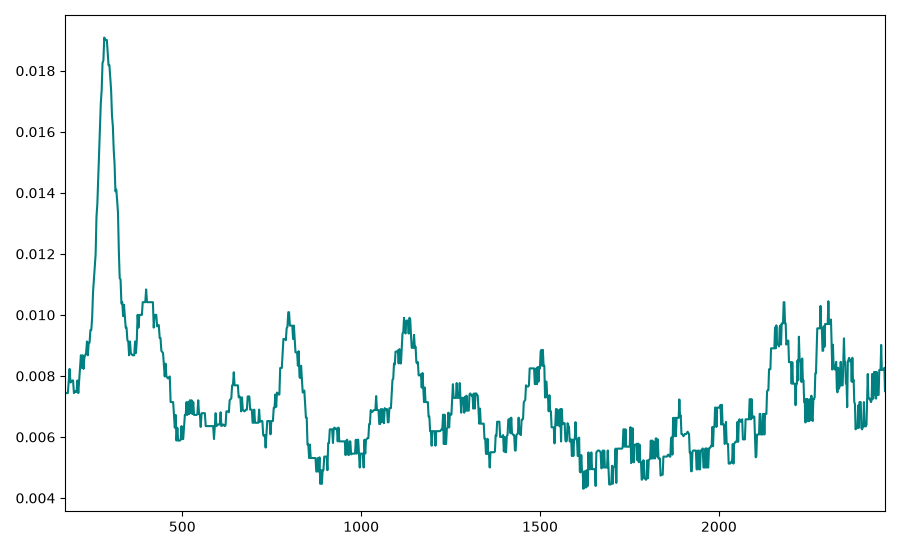
\includegraphics[width=0.7\textwidth]{plots/unknown_2.png}
    \caption{Spectra of \textit{unknown sample 2}}
    \label{fig:unknown_2}
\end{figure}
% }}}2
% Ethanol {{{2
\subsection{Ethanol concentration of an unknown sample}

Spectra of multiple samples with known ratios of ethanol and destilled water were recorded during the experiment and are shown in figures \ref{fig:water}, \ref{fig:ethanol_50}, \ref{fig:ethanol_75}, and \ref{fig:ethanol_100}.



\begin{figure}[H]
    \centering
    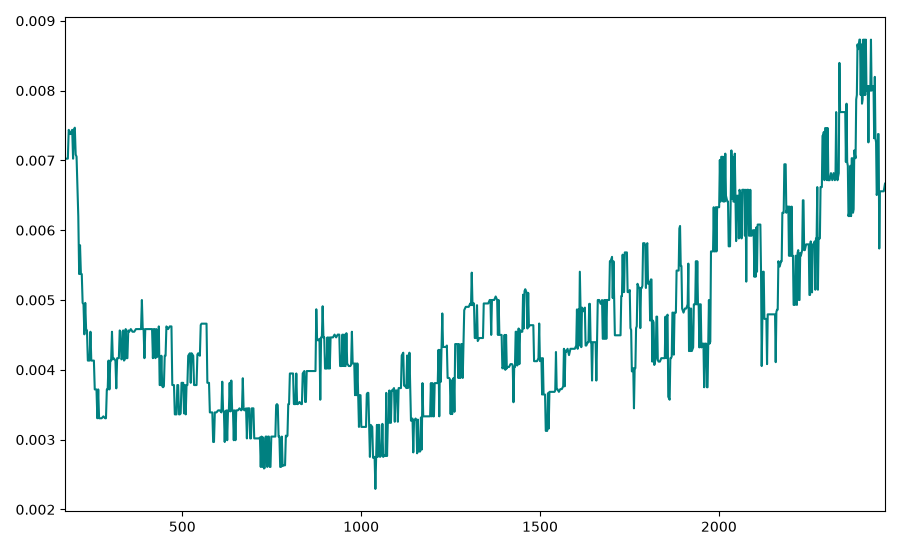
\includegraphics[width=0.7\textwidth]{plots/water.png}
    \caption{Spectra of destilled water.}
    \label{fig:water}
\end{figure}

\begin{figure}[H]
    \centering
    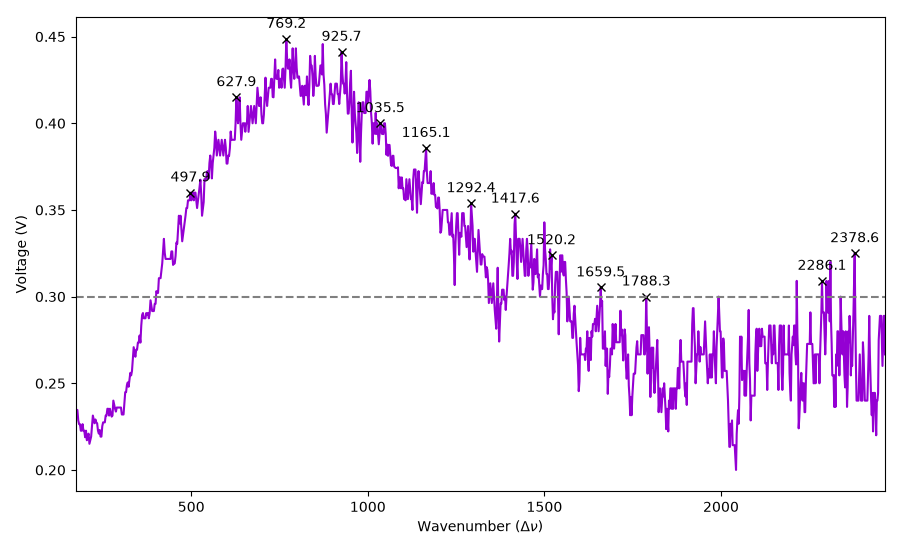
\includegraphics[width=0.7\textwidth]{plots/ethanol_50.png}
    \caption{Spectra of ethanol at $50\%$}
    \label{fig:ethanol_50}
\end{figure}

\begin{figure}[H]
    \centering
    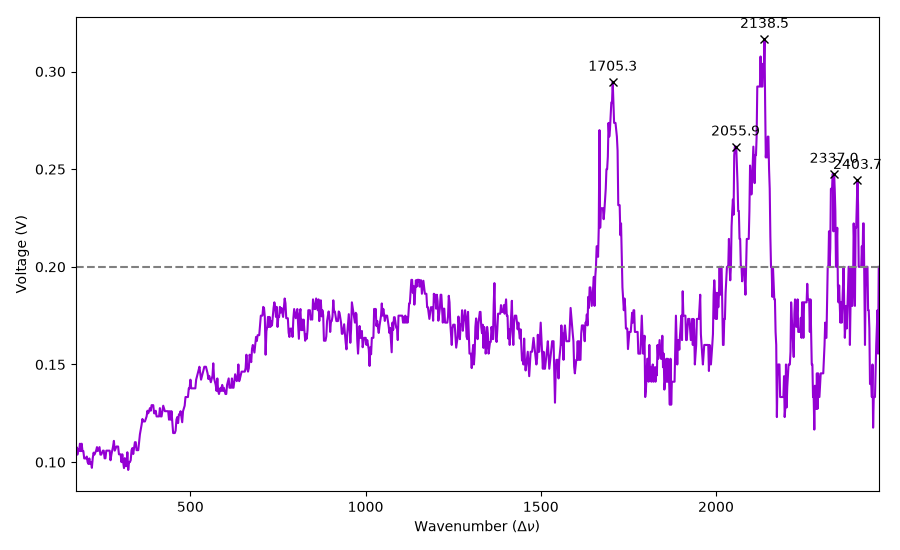
\includegraphics[width=0.7\textwidth]{plots/ethanol_75.png}
    \caption{Spectra of ethanol at $75\%$}
    \label{fig:ethanol_75}
\end{figure}

\begin{figure}[H]
    \centering
    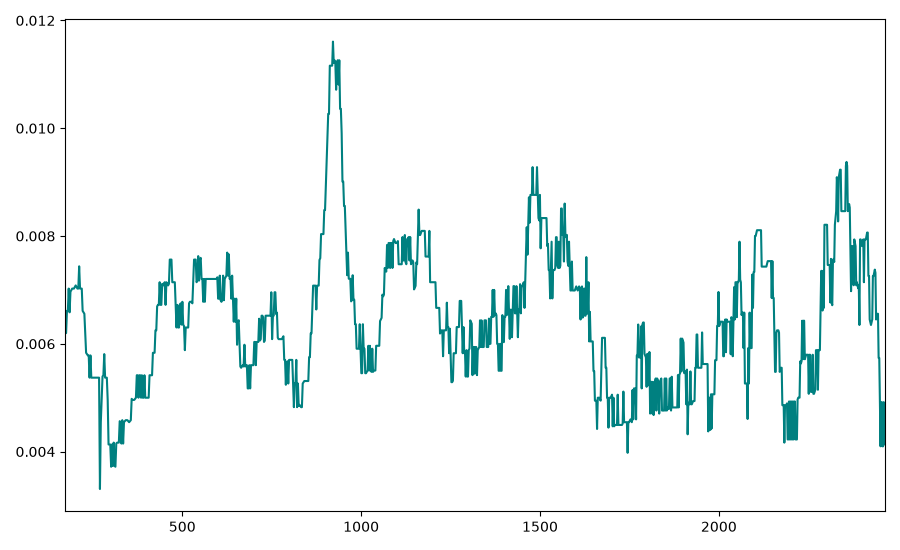
\includegraphics[width=0.7\textwidth]{plots/ethanol_100.png}
    \caption{Spectra of ethanol at $100\%$}
    \label{fig:ethanol_100}
\end{figure}
% }}}2
% FITS {{{2
\subsection{Fit of relevant peaks}
%%%%%%%%%%%%%%%%%%%%CCL4%%%%%%%%
\subsubsection{CCL4}
%BIG PEAK
\begin{figure}[H]
    \centering
    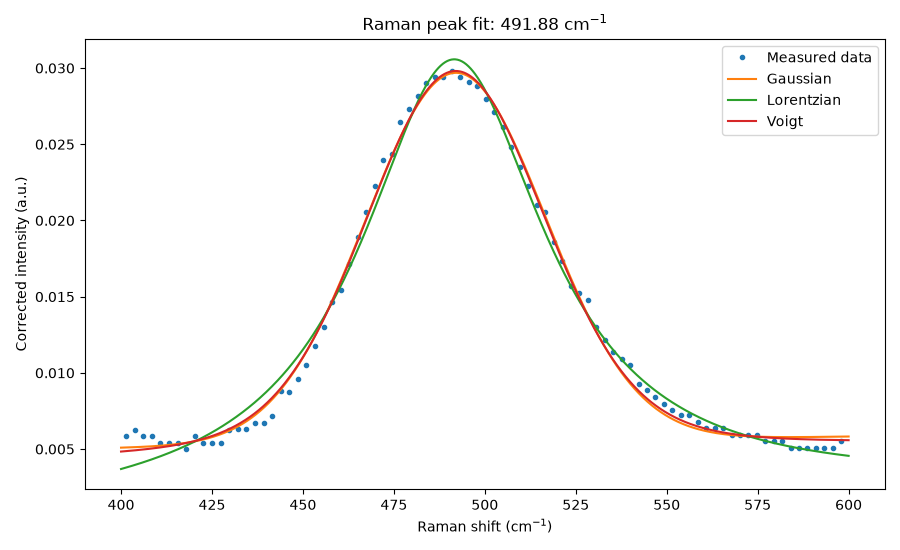
\includegraphics[width=0.9\textwidth]{plots/CCL4_458.png}
    \caption{Fit for  Raman peak at $\SI{491.9}{\cm ^{-1}}$}
    \label{fig:ccl4_458}
\end{figure}
\begin{table}[H]
\centering
\begin{tabular}{rllllll}
\toprule
Peak & Fit & $\Delta\nu$ (cm$^{-1}$) & $\lambda$ (nm) & FWHM (cm$^{-1}$) & $R^2$ \\
\midrule
491 & Gaussian & 492.0 ± 0.2 & 653.35 ±  0.01 & 58.2 & 0.9954 \\
491 & Lorentzian & 491.4 ± 0.3 & 653.32 ±  0.01 & 61.8 & 0.9902 \\
491 & Voigt & 491.9 ± 0.2 & 653.34 ±  0.01 & 58.8 & 0.9956 \\
\bottomrule
\end{tabular}
\caption{Fit parameters for the $\SI{491.9}{\cm^{-1}}$ Raman peak.}
\end{table}
%TWIN PEAKS OR WHATEVER

\begin{figure}[H]
    \centering
    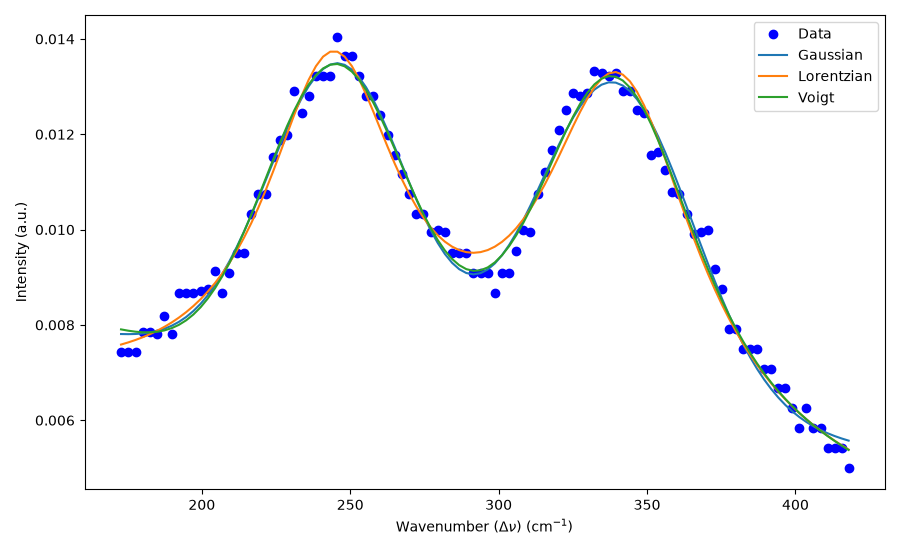
\includegraphics[width=0.9\textwidth]{plots/dual_peak.png}
    \caption{Fit for  Raman peak at $\SI{491.9}{\cm ^{-1}}$}
    \label{fig:ccl4_dual}
\end{figure}
\begin{table}[H]
\centering
\begin{tabular}{rllllll}
\toprule
Peak & Fit & $\Delta\nu$ (cm$^{-1}$) & FWHM (cm$^{-1}$) & $R^2$ \\
\midrule
245 & Gaussian & 246.2 $\pm$ 0.5 & 56.0 & 0.9838 \\
332 & Gaussian & 339.0 $\pm$ 0.4 & 62.0 & 0.9838 \\
245 & Lorentzian & 244.2 $\pm$ 0.5 & 56.1 & 0.9806 \\
332 & Lorentzian & 340.5 $\pm$ 0.5 & 64.4 & 0.9806 \\
245 & Voigt & 245.0 $\pm$ 0.6 & 52.4 & 0.9848 \\
332 & Voigt & 338.7 $\pm$ 0.8 & 67.5 & 0.9848 \\
\bottomrule
\end{tabular}
\caption{Fit parameters for the twin peaks $\SI{245}{\cm^{-1}}$ and $\SI{332}{\cm^{-1}}$ Raman peak.}
\end{table}


\begin{figure}[H]
    \centering
    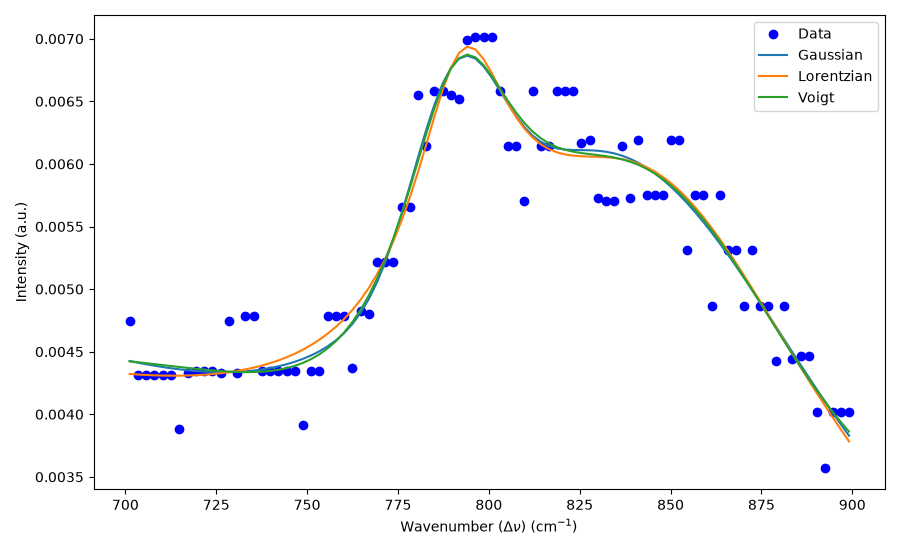
\includegraphics[width=0.9\textwidth]{plots/fermi_resonance.png}
    \caption{Fit for fermi resonance}
    \label{fig:ccl4_fermi}
\end{figure}
\begin{table}[H]
\centering
\begin{tabular}{rllllll}
\toprule
Peak & Fit & $\Delta\nu$ (cm$^{-1}$) & FWHM (cm$^{-1}$) & $R^2$ \\
\midrule
780 & Gaussian & 791.1 $\pm$ 1.2 & 28.3 & 0.9212 \\
830 & Gaussian & 835.5 $\pm$ 4.5 & 105.5 & 0.9212 \\
780 & Lorentzian & 792.9 $\pm$ 1.2 & 33.6 & 0.9179 \\
830 & Lorentzian & 845.1 $\pm$ 4.4 & 121.5 & 0.9179 \\
780 & Voigt & 791.6 $\pm$ 1.4 & 41.6 & 0.9215 \\
830 & Voigt & 843.5 $\pm$ 4.6 & 65.7 & 0.9215 \\
\bottomrule
\end{tabular}
\caption{Fit parameters for the twin peaks $\SI{245}{\cm^{-1}}$ and $\SI{332}{\cm^{-1}}$ Raman peak.}
\end{table}


%%%%%%%%%%%%%%BENZENE%%%%%%%%%%%%%%%%%%
\subsubsection{Benzene}
\begin{figure}[H]
    \centering
    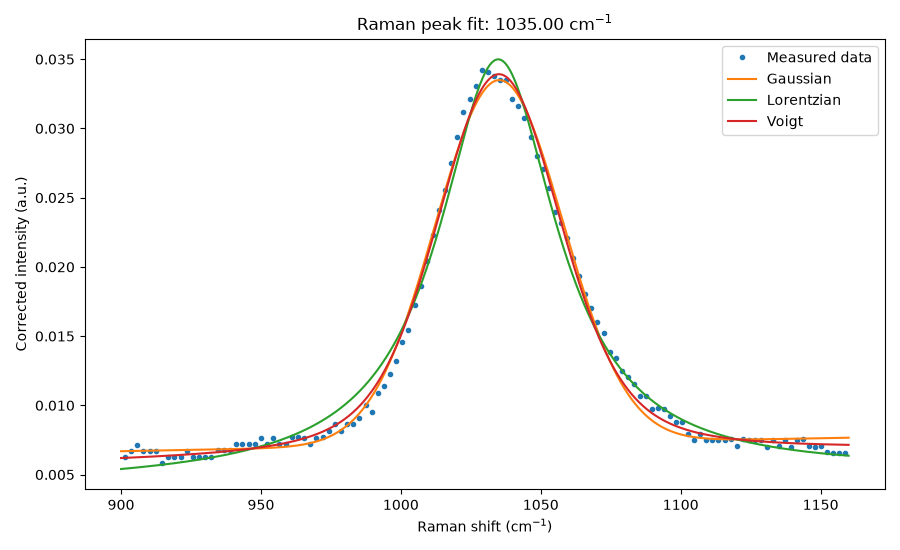
\includegraphics[width=0.9\textwidth]{plots/Benzene_991.png}
    \caption{Fit for  Raman peak at $\SI{1035}{\cm ^{-1}}$}
    \label{fig:ccl4_991}
\end{figure}
\begin{table}[H]
\centering
\begin{tabular}{rllllll}
\toprule
Peak & Fit & $\Delta\nu$ (cm$^{-1}$) & $\lambda$ (nm) & FWHM (cm$^{-1}$) & $R^2$ \\
\midrule
1028 & Gaussian & 1035.1 ± 0.2 & 677.38 ±  0.01 & 53.8 & 0.9934 \\
1028 & Lorentzian & 1034.7 ± 0.3 & 677.37 ±  0.01 & 51.4 & 0.9892 \\
1028 & Voigt & 1035.0 ± 0.2 & 677.38 ±  0.01 & 53.2 & 0.9950 \\
\bottomrule
\end{tabular}
\caption{Fit parameters for the Benzene $\SI{1035}{\cm^{-1}}$ Raman peak.}
\end{table}
% }}}2
% }}}1
% Discussion {{
\section{Discussion}
\subsection{CCl4}
Taking a closer look at the CCL4 spectra above, notice that not all of the laser/analyzer configurations yield expected results. If we consider exclusively the sample and the relative orientation of the incident polarization and analyzer, we would expect a simmetrical behavior of the experiment configurations. CCL4 has totally symmetric $A$ modes and non-symmetric $F$ modes.

If we simplify the experiment to two orthogonal polarization directions $x$ and $y$, we can think of the experiment yielding symmetric results as in table \ref{tab:ccl4_polarization}. This is however not the case. In reality, the experiment doesn't yield the expected symmetry but instead the ones shown in table \ref{tab:ccl4_polarization_real}.

Give that CCL4 is an isotropic sample, there is no molecular reason for this to dissapear while the other survives. The most likely explanation is that the optical system has an additional polarization-dependent transmission/collection effect. As already mentioned, the monochromator used in the experiment has a different response to the orientation of light. This conbined with an improper optical aligment is one likely explanation as to why we cannnot resolve the lines with the analizer at the $0^{\circ}$ degrees configuration.
\begin{table}[H]
    \centering
    \caption{Idealized polarization dependence of Raman scattering in an isotropic
    $\mathrm{CCl_4}$ sample. The $A_1$ mode produces polarized scattering,
    while the $F_2$ modes produce depolarized scattering.}
    \label{tab:ccl4_polarization}
    \begin{tabular}{c|cc}
        & \multicolumn{2}{c}{Analyzer polarization} \\
        Laser polarization & $0^\circ$ & $90^\circ$ \\
        \hline
        $0^\circ$  & $A_1$ & $F_2$ \\
        $90^\circ$ & $F_2$ & $A_1$ \\
    \end{tabular}
\end{table}

\begin{table}[H]
    \centering
    \caption{Results of the experiment}
    \label{tab:ccl4_polarization_real}
    \begin{tabular}{c|cc}
        & \multicolumn{2}{c}{Analyzer polarization} \\
        Laser polarization & $0^\circ$ & $90^\circ$ \\
        \hline
        $0^\circ$  & noise & $F_2$ \\
        $90^\circ$ & noise & $A_1$ \\
    \end{tabular}
\end{table}
To discuss the number of frencuency shifts in our spectra, it's relevant to explain the molecular structure of CCL4 and its possible vibrational modes. A very didactic animation can be found on \cite{chalmers}(\href{https://fy.chalmers.se/OLDUSERS/brodin/MolecularMotions/CCl4modes.html}{click here}). A diagram is also sketched for those who are not reading this report on an e-device.


\begin{figure}[H]
    \centering
    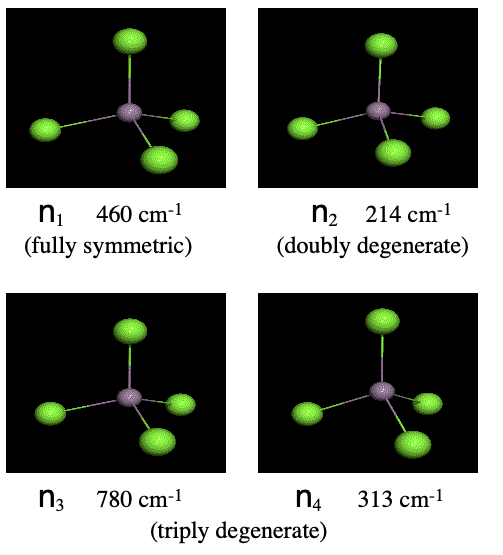
\includegraphics[width=0.6\textwidth]{plots/modes.png}
    \caption{Vibrational modes of Carbon tetrachloride. Adapted from \cite{chalmers}}
    \label{fig:ccl4_modes}
\end{figure}

Each of these vibrational modes influences the amount of lines seen in the raman spectra.

%%%REVIEW

The vibrational modes of $\mathrm{CCl_4}$ can be classified according to the symmetry of the molecule, resulting in four distinct fundamental modes: $\nu_1(A_1)$, $\nu_2(E)$, $\nu_3(F_2)$, and $\nu_4(F_2)$.Consequently, four distinct fundamental vibrational frequencies are expected in the Raman spectrum, and are indeed seen in figure \ref{fig:CCL4_90_90}, although the peak corresponding to $\nu_{3}$ is barely perceptible in our measurements.

Peak $\nu_{3}$ corresponds to a fermi resonance. Because of this, instead of observing a sigle peak, we see a double peak profile in figure \ref{fig:ccl4_peaks}. This is why the fit shown in figure \ref{fig:ccl4_fermi} accounts for a two peak fit, even if in our data this distinction is not percieved.

\begin{figure}[H]
    \centering
    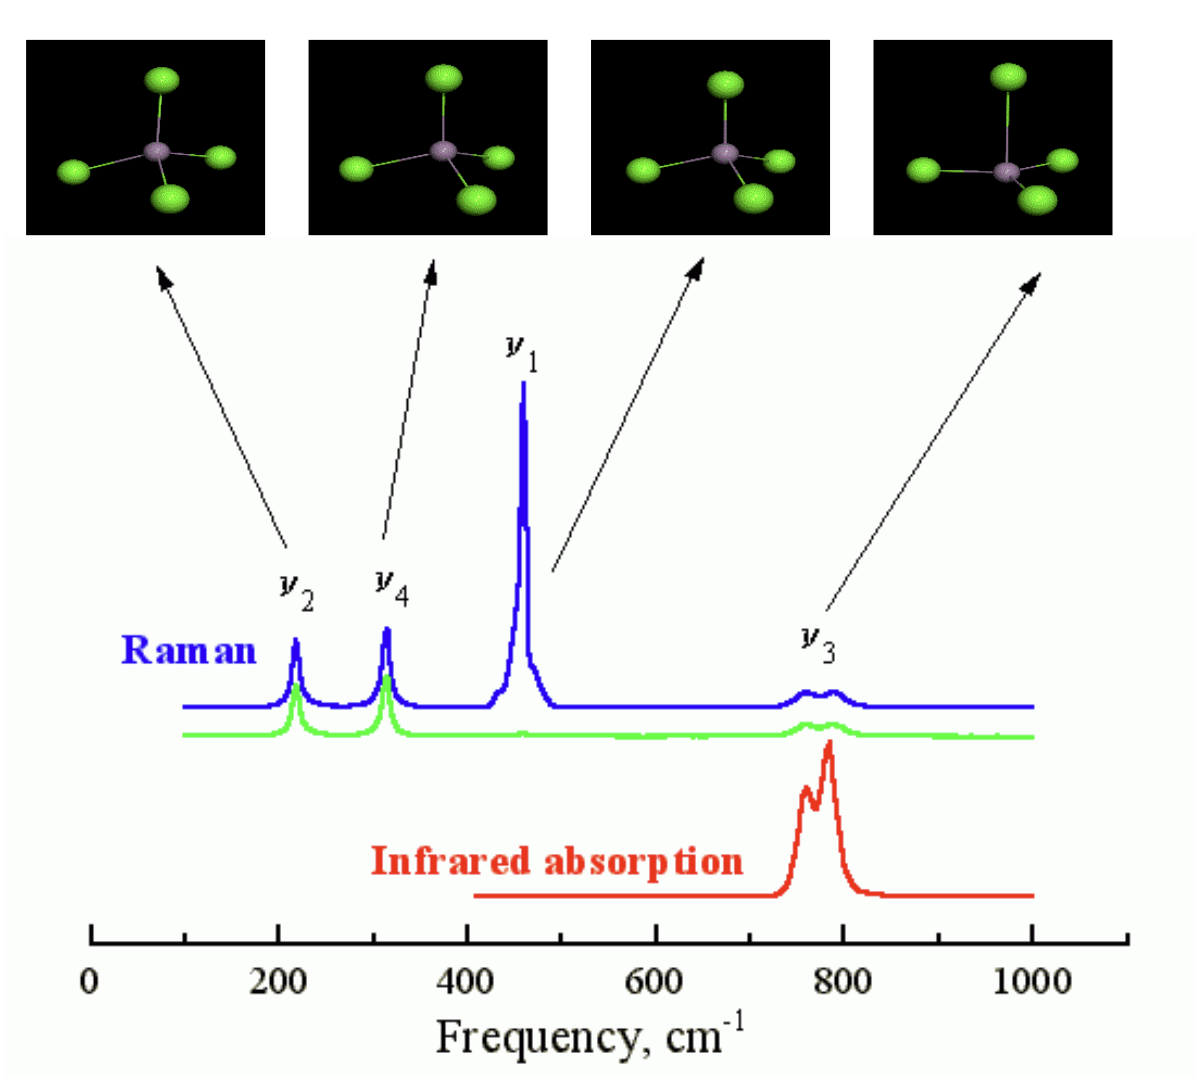
\includegraphics[width=0.6\textwidth]{plots/Spectra_modes.png}
    \caption{Raman peaks corresponding to vibrational modes. Adapted from \cite{chalmers}}
    \label{fig:ccl4_peaks}
\end{figure}



For tables \ref{tab:ccl4_raman_comparison} and \ref{tab:benzene_raman_comparison}, the following notation is useful: $C = 3 \sim 6\si{cm^{-1}}$,$E = 15 \sim 30 \si{cm^{-1}}$,


As it is shown on the mentioned tables, our measurements are off by a few dozens of wavenumbers. Most likely the reference between the software/monochromator was not properly adjusted before the measurments. and hence a displacement of wavenumbers occured in our data.

\begin{table}[htbp]
    \centering
    \caption{Literature and measured Raman bands of carbon tetrachloride ($\mathrm{CCl_4}$).}
    \label{tab:ccl4_raman_comparison}
    \begin{tabular}{cccccc}
        \hline
        Symmetry & Mode & NIST $\nu$ &
        Uncertainty & Measured $\nu$ & Deviation \\
        & & \si{\per\centi\meter} & \si{\per\centi\meter} &
        \si{\per\centi\meter} & \si{\per\centi\meter} \\
        \hline
        $a_1$ & Symmetric stretch &
        458.7 & C & 490.9 &  32.2 \\

        $e$ & Degenerate deformation &
        217.0 & C & 245.7 & 28.7 \\

        $f_2$ & Degenerate stretch &
        790.4 & E & 798.5 & 8.1 \\

        $f_2$ & Degenerate stretch &
        761.7 & E & -- & -- \\

        $f_2$ & Degenerate deformation &
        313.5 & C & 332.3 & 18.8 \\
        \hline
    \end{tabular}
\end{table}
\subsubsection{polarization of CCL4 modes}

\begin{figure}[H]
    \centering
    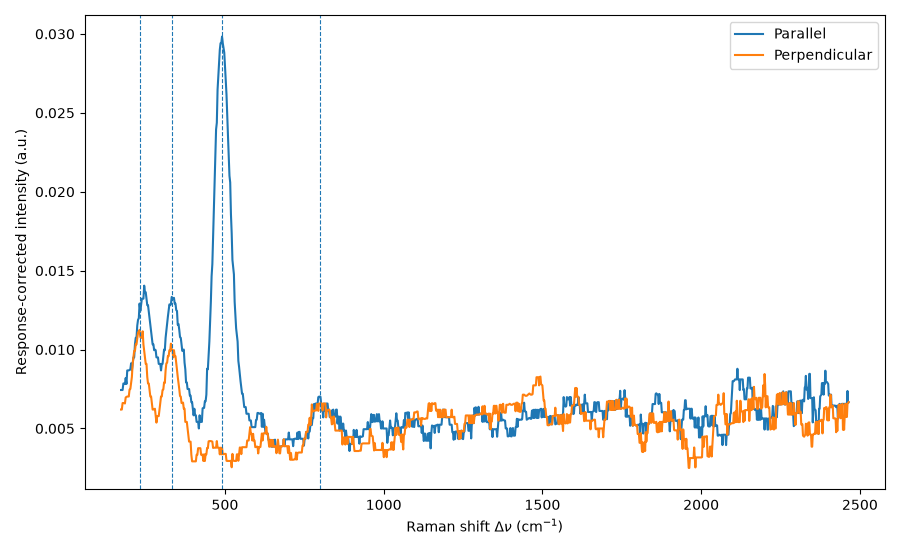
\includegraphics[width=0.8\textwidth]{plots/CCL4_imposed.png}
    \caption{Horizontal and Perpendicular measurements superimposed}
    \label{fig:ccl4_imposed}
\end{figure}



\begin{table}[H]
\centering
\begin{tabular}{rlll}
\toprule
$\Delta\nu$ (cm$^{-1}$) & $I_\parallel$ (a.u.) & $I_\perp$ (a.u.) & $\rho$ \\
\midrule
231 & 0.0132 & 0.0112 & 0.851 \\
332 & 0.0133 & 0.0104 & 0.778 \\
490 & 0.0298 & 0.00378 & 0.127 \\
798 & 0.00702 & 0.00658 & 0.937 \\
\bottomrule
\end{tabular}
\caption{polarization ratios for the vibrational modes of CCL4}
\label{tab:ccl4_pol}
\end{table}
Table \ref{tab:ccl4_pol} shows the calculated polarization ratios from the measurements taken. Our measurements are in agreement with the literature reported in \cite{NIST}. The only strongly polarized peak corresponds to the vibrational mode $\nu(A_1)$, since it corresponds to a diagonal entry in the raman polarization tensor of CCL4. The rest of the peaks $\nu_2$, $\nu_3$ and $\nu_3$ correspond to non-diagonal entries in the tensor, and are thus depolarized as seen in both figure \ref{fig:ccl4_imposed} and table \ref{tab:ccl4_pol}


\subsection{Benzene}
\subsection{CCL4 and Benzene}

\subsubsection{peaks}
Tables \ref{tab:ccl4_raman_comparison} and \ref{tab:benzene_raman_comparison} show the reported raman shifts according to  \cite{NIST} against the measured shifts in the experiment.

FFor Benzene, we were able to record only the most promiment peak, located at $\SI{991.6}{cm^{-1}}$. The rest of the peaks are labeled in the literature (see \cite{NIST}) as medium or low intensity peaks. As mentioned, our alignment was not providing a precise input scattered beam to the monochromator, so little intensity for the raman peaks of benzene was obtained.
\begin{table}[htbp]
    \centering
    \caption{Literature and measured Raman bands of Benzene ($\mathrm{C_6H_6}$)}
    \label{tab:benzene_raman_comparison}
    \begin{tabular}{cccccc}
        \hline
        Symmetry & Mode & NIST $\nu$ &
        Uncertainty & Measured $\nu$ & Deviation \\
        & & \si{\per\centi\meter} & \si{\per\centi\meter} &
        \si{\per\centi\meter} & \si{\per\centi\meter} \\
        \hline
        $a_{1g}$ & CH stretch &
        3061.9 & C & -- & -- \\

        $a_{1g}$ & Ring stretch &
        991.6 & C & 1028.9 & 37.3 \\

        $a_{2g}$ & CH bend &
        1326.0 & E & -- & -- \\

        $e_{1g}$ & CH bend &
        848.9 & C & -- & -- \\

        $e_{2g}$ & CH stretch &
        3046.8 & C & -- & -- \\

        $e_{2g}$ & Ring stretch &
        1606.4 & E & -- & -- \\

        $e_{2g}$ & Ring stretch &
        1584.6 & E & -- & -- \\

        $e_{2g}$ & CH bend &
        1178.0 & C & -- & -- \\

        $e_{2g}$ & Ring deformation &
        605.6 & C & -- & -- \\
        \hline
    \end{tabular}
\end{table}
\subsubsection{peak polarization}
By observing figures \ref{fig:CCL4_0_90} and \ref{fig:CCL4_90_90}, it is evident that the peak we measured at \SI{490.9}{\centi\meter ^{-1}} corresponds to strongly polarised Raman scattering. Approximating from the values recorded
\begin{equation}
	\rho = \frac{I_\perp}{I_\parallel} \approx \frac{0.004}{0.030} = 0.13
\end{equation}
comparing with what was discussed in section \ref{sec:depol}, is is indeed strongly polarized.



The rest of the peaks recorded for CCL4 are not strongly polarized, and from the graphs it can be estimated that $\rho \ge \frac{3}{4}$ for these.

Similarly, the only peak measured for benzene is only really visible on figure \ref{fig:benzene_90_90} which indicates strong polarization without any calculation needed.

\cite{NIST} also reports the same polarization degrees as in our experiment

\subsection{unknown samples}
The spectra of both unknown samples was taken without the analyzer, so the depolarization ratio cannot be discussed.

To find out what molecule(s) are in the sample, the \href{https://webbook.nist.gov/chemistry/vib-ser/}{
Search for Species Data by Vibrational Energy Value} of the NIST was used.
After introducing the wavenumbers recorded in the experiment, a comparison between many molecules was done. given that we're lacking the polarization of the peaks, it's harder to pinpoint the actual content of the cuvette. Many molecules and peaks were looked after and a lot of the search filters were applied. Ultimately, we suspect that our spectra is heavily shifted, and we couldn't identify either of the two samples.

If we dismiss the assumption that the spectra is shifted, then the spectra for sample 1 (figure \ref{fig:unknown_1}) contains two of the strong peaks of Borine carbonyl $\mathrm{CH_3^{11}BO}$, albeit slightly shifted from where they should be ($\SI{2380}{\cm^{-1}}$ recorded at $\SI{2384}{\cm^{-1}}$ and $\SI{2169}{\cm^{-1}}$ recorded at $\SI{2145}{\cm^{-1}}$). However, the second value is still far enough to classify it as such.


Regarding the second sample, it was originally thought the peaks looked similar to bromoform raman peaks, but upon further inspection, the relative intensities between peaks do not match.

We conclude this discussion suggesting that narrowing down the sample would've been easier if polarization data had been recorded during the experiment, as well as a more careful alignment of the analog/software calibration of the wavenumber.


\subsection{Determination of the ethanol concentration of an unknown sample}

Upon further inspection, we notice that all of the ethanol samples (Figures \ref{fig:water} to \ref{fig:ethanol_100}) show no clear correlation between peak intensities or position. It is unclear how to proceed to make this four spectra a ruler for ethanol concentration in unknown samples. Adding the fact that most likely our unknown spectra is heavily shifted, we opted to avoid making poorly-founded calculations of ethanol concentration.
% }}}
% References printout {{{
\nocite{*}
\newpage
% ============================================================

\bibliographystyle{unsrtnat}
\bibliography{references}
% }}}
\end{document}

